\documentclass[a4paper, 10pt, draft]{report}

\usepackage{ucs}
\usepackage[utf8x]{inputenc}
\usepackage[english]{babel}
\usepackage[T1]{fontenc}
\usepackage{ae, aecompl}

\usepackage{amsmath}
\usepackage{amssymb}
\usepackage{bussproofs}
\usepackage{semantic}
\usepackage{listings}
\usepackage{color}
\usepackage{tabularx} % Kindla laiusega tabelid
\newcolumntype{C}{>{\centering\arraybackslash}X}
\usepackage{multirow} % lahtrid mitmes veerus/reas
\usepackage{setspace}
\usepackage{longtable}
\usepackage{tikz}

\DeclareMathOperator*{\basis}{basis}
\DeclareMathOperator*{\goodguard}{goodguard}
\DeclareMathOperator*{\goodexpr}{goodexpr}
\DeclareMathOperator*{\env}{env}
\DeclareMathOperator*{\up}{up}
\DeclareMathOperator*{\lo}{lo}
\DeclareMathOperator*{\newloc}{newloc}
\DeclareMathOperator*{\force}{\mathit{force}}
\DeclareMathOperator*{\noforce}{\mathit{noforce}}
\newcommand{\mycode}[1]{\ensuremath{\mbox{\lstinline{#1}}}}
\newcommand{\cast}[1]{\ensuremath{\mycode{cast}_{#1}}}

% Literaalid:
\newcommand{\litQuote}[1]{\textcolor{black}{\texttt{'#1'}}}
%\newcommand{\litQuote}[1]{\textcolor{blue}{\texttt{'#1'}}}

% BNF
\newcommand{\grammarRules}[1]{\small{\singlespacing\vspace{-2em}\begin{align*}#1\end{align*}}}
\newcommand{\bnfNT}[1]{\ensuremath{\mathbf{\left\langle\mbox{\texttt{#1}}\right\rangle}}}
\newcommand{\bnfT}[1]{\ensuremath{\mbox{\litQuote{#1}}}}
\newcommand{\bnfM}[1]{\ensuremath{\mbox{\textcolor{black}{\texttt{\uppercase{#1}}}}}} % Makro
%\newcommand{\bnfM}[1]{\ensuremath{\mbox{\textcolor{darkgray}{\texttt{\uppercase{#1}}}}}} % Makro

% Regex
\newcommand{\regexAlt}[1]{\ensuremath{\left[\mbox{\litQuote{#1}}\right]}}

\newcommand{\anyop}{\ensuremath{\circledast}}
\newcommand{\myop}[2]{\ensuremath{\operatorname{#1}\!\left(#2\right)}}
\newcommand{\mybinaryop}[3]{\ensuremath{\operatorname{#1}\!\left(#2, #3\right)}}
\mathlig{|->}{\mapsto}
\mathlig{*=}{\ \mbox{*=}\ }
\mathlig{/=}{\ \mbox{/=}\ }
\mathlig{+=}{\ \mbox{+=}\ }
\mathlig{-=}{\ \mbox{-=}\ }

\lstset{language=C}
\lstset{tabsize=4}
\lstset{mathescape=true}
\lstset{basicstyle=\ttfamily}

\title{The Formal Semantics of the SecreC Language}
\date{\today}
\author{{Jaak Randmets}, {Jaak Ristioja}}

\begin{document}

\maketitle

\newpage
\chapter{Grammar}\label{sec:grammar}

SecreC is a domain-specific programming language strongly influenced by the
syntax of C. Since it is aimed at providing a higher-level language for writing
computer programs for the Sharemind hybrid virtual machine, SecreC needs to be
fully formalized to provide strong security guarantees in the future.

The grammar given in this chapter does not exactly describe the language
accepted by the current SecreC compiler described in \cite{SECREC}. Major
omissions in this paper is type casting which is still being worked on.
Compared to \cite{SECREC}, we allow global variable definitions and procedure
definitions to occur in any order. Also, specifying the SecreC standard library
is not a part of this document.

We specify the syntax for the subset of SecreC using a context free grammar.
The grammar rules are described using a variant of the Backus-Naur Form (BNF)
extended with some regular expression constructs, such as regular braces for
grouping subexpressions, the repetition operator $*$ as superscript, and the
$?$ suffix for denoting optionality of the preceding subexpression.

In the specification of the grammar, we are using angle brackets to denote
\bnfNT{nonterminals}, apostrophes to denote terminals, e.g., \bnfT{exact
strings} as returned by the scanner, and all capitals for certain sets of
strings such as the set of \bnfM{IDENTIFIER} names.

\section{Character set and whitespace}\label{sec:grammar:chars}

Tokens returned by the SecreC scanner are either keywords, operators, string
literals, integer literals, unsigned integer literals or identifiers. When
tokenizing the input, whitespace is allowed to appear between tokens. There are
also two kinds of comments which are treated as whitespace between tokens. Any
such whitespace is ignored, except inside string literals. Inside string
literals, whitespace and characters denoting comment constructs are returned as
part of the string literal token.

In SecreC, there are 22 keywords: \mycode{bool}, \mycode{break},
\mycode{continue}, \mycode{declassify}, \mycode{do}, \mycode{else},
\mycode{false}, \mycode{for}, \mycode{if}, \mycode{int}, \mycode{private},
\mycode{public}, \mycode{return}, \mycode{string}, \mycode{true},
\mycode{unsigned}, \mycode{void}, \mycode{while}, \mycode{size},
\mycode{shape}, \mycode{reshape} and \mycode{cat}; and 28 other tokens with
fixed contents:

\begin{center}
\begin{tabular}{ccccccc}
    \mycode{+=} & \mycode{-=} & \mycode{*=} & \mycode{/=} & \mycode{\%=} & \mycode{&&} & \mycode{||} \\
    \mycode{=}  & \mycode{<=} & \mycode{>=} & \mycode{<}  & \mycode{>}   & \mycode{==} & \mycode{!=} \\
    \mycode{\{} & \mycode{\}} & \mycode{(}  & \mycode{)}  & \mycode{?}   & \mycode{:}  & \mycode{,} \\
    \mycode{+}  & \mycode{*}  & \mycode{/}  & \mycode{\%} & \mycode{-}   & \mycode{!}  & \mycode{;}
\end{tabular}
\end{center}

String literals (strings in the set \bnfM{STRING\_LITERAL}) in SecreC are
tokens which start with a double quote character (") and continue up to (and
including) another double quote character not preceded by a backslash character
(\textbackslash). The string literal therefore always ends and starts with
double quote characters and may contain \textit{escape sequences}, e.g.,
\textbackslash " to denote a single double quote character in the string and
\textbackslash\textbackslash\ denoting a single backslash in the string. The
string corresponding to the string literal is stripped of the two enclosing
double quotes, and has the escape sequences replaced by their single-character
counterparts. Implementation may also define additional escape sequences.

Integer literals (strings in the set \bnfM{INT\_LITERAL}) in SecreC are tokens
which are used to represent signed integer values in the source code of SecreC
programs. These are required to match the following regular expression:
\[ 0\ | \left(1\ |\ 2\ |\ 3\ |\ 4\ |\ 5\ |\ 6\ |\ 7\ |\ 8\ |\ 9\right)\left(0\ |\ 1\ |\ 2\ |\ 3\ |\ 4\ |\ 5\ |\ 6\ |\ 7\ |\ 8\ |\ 9\right)^{*}\]

Unsigned integer literals (strings in the set \bnfM{UINT\_LITERAL}) are used to
represent unsigned integer values and are required to match the following
regular expression:
\[ 0 \left(0\ | \left(1\ |\ 2\ |\ 3\ |\ 4\ |\ 5\ |\ 6\ |\ 7\ |\ 8\ |\ 9\right)\left(0\ |\ 1\ |\ 2\ |\ 3\ |\ 4\ |\ 5\ |\ 6\ |\ 7\ |\ 8\ |\ 9\right)^{*}\right) \]

Identifiers (string in the set \bnfM{IDENTIFIER}) are tokens which represent
variable and procedure names in SecreC. These strings consist only of lowercase
and uppercase Latin characters, underscores and decimal digits, the first
character of any identifier must not be a decimal digit. Keywords are not
considered to be identifiers.

There are two types of comments in SecreC, both of which should not be included
in the output list of tokens. The single line comments start with two
consecutive forward slashes (//) and continue until a new line character (e.g.
bytes with hexadecimal values 0x0A and 0x0D in ASCII). Multiline comments start
with a consecutive forward slash and asterisk (/*) and continue up to (and
including) a consecutive asterisk and forward slash (*/). If the character
sequences that start comments appear inside string literals or other comments,
they are not considered to start comments. This also means that comments can
not be nested inside other comments.

\section{Program}\label{sec:grammar:program}
The top-level of any SecreC program consists of one or more global variable or
procedure definitions:
\grammarRules{
  \bnfNT{program} ::=&\ \bnfNT{variable\_definition}\ \bnfNT{program} \\
                    |&\ \bnfNT{procedure\_definition}\ \bnfNT{program} \\
                    |&\ \bnfNT{variable\_definition} \\
                    |&\ \bnfNT{procedure\_definition}
}

Later static checking rules require that there be at least a procedure called
\mycode{main} present in the program. Note that while variable definitions can
also appear in local scopes, procedures can only be defined globally, under the
\bnfNT{program} nonterminal rule. According to the semantics of SecreC, all
definitions after the definition of procedure \mycode{void main()} are
unreachable.  The static checking rules and semantics for the top-level program
constructs are given in detail in Subsection \ref{sec:checking:typing:programs}
and Section \ref{sec:semantics:program}, respectively.

\subsection{Variable definitions}\label{sec:grammar:vardef}

All variable are declared by specifying the type of the variable, its name and
optionally the sizes of dimensions:
\grammarRules{
  \bnfNT{variable\_declaration} ::= \ \bnfNT{type\_specifier}\ \bnfM{IDENTIFIER}\ \bnfNT{dimensions}?
}
where dimensions are given by comma separated expressions between brackets:
\grammarRules{
  \bnfNT{dimensions} ::=&\ \bnfT{[}\ \bnfNT{expression\_list}?\ \bnfT{]}\\
  \bnfNT{expression\_list} ::=&\ \bnfNT{expression}\ \bnfT{,}\ \bnfNT{expression\_list} \\
                            |&\ \bnfNT{expression}
}

Variables are defined by declaring them and optionally initializing them:
\grammarRules{
  \bnfNT{variable\_definition}  ::=&\ \bnfNT{variable\_declaration}\ \bnfT{=}\ \bnfNT{expression}\ \bnfT{;} \\
                                  |&\ \bnfNT{variable\_declaration}\ \bnfT{;} }

\section{Types}\label{sec:grammar:types}

Type annotations in SecreC consist of the possible security type annotation,
followed by the data type annotation and optionally dimensionality annotation:
\grammarRules{
  \bnfNT{type\_specifier} ::=&\ \bnfNT{sectype\_specifier}? \\
                             &\ \bnfNT{datatype\_specifier} \\
                             &\ \bnfNT{dimensionality\_specifier}? \\
  \bnfNT{sectype\_specifier} ::=&\ \bnfT{public}\ |\ \bnfT{private} \\
  \bnfNT{datatype\_specifier} ::=&\ \bnfT{string}\ |\ \bnfT{int}\ |\ \bnfT{unsigned}\ \bnfT{int}\ |\ \bnfT{bool} \\
  \bnfNT{dimensionality\_specifier} ::=&\ \bnfT{[}\ \bnfT{[}\ \bnfM{INT\_LITERAL}\ \bnfT{]}\ \bnfT{]}
}

\section{Procedures}\label{sec:grammar:procedures}

Procedure definitions consist of a return type annotation, the name of the
procedure, its list of type-annotated parameters and the function body:
\grammarRules{
  \bnfNT{procedure\_definition} ::=&\ \left(\bnfT{void}\ |\ \bnfNT{type\_specifier}\right)\ \bnfM{IDENTIFIER} \\
                                   &\ \bnfT{(}\ \bnfNT{procedure\_parameter\_list}?\ \bnfT{)} \\
                                   &\ \bnfNT{compound\_statement} \\
  \bnfNT{procedure\_parameter\_list} ::=&\ \bnfNT{procedure\_parameter}\\
                                        &\ \left( \bnfT{,}\ \bnfNT{procedure\_parameter} \right)^{*} \\
  \bnfNT{procedure\_parameter} ::=&\ \bnfNT{type\_specifier}\ \bnfM{IDENTIFIER}
}

Note, that if the procedure does not return anything, its return type should be
annotated as \bnfT{void}. The body of the procedure is always enclosed in curly
brackets (i.e. \bnfT{\{} and \bnfT{\}}) because of \bnfNT{compound\_statement}.



\section{Statements}\label{sec:grammari:statements}

The set of statements in SecreC is also similar to those in C, except that
there are no \mycode{switch} statements, \mycode{goto} statements and labels.
Statements may only appear inside procedure bodies.
\grammarRules{
  \bnfNT{compound\_statement} ::=&\ \bnfT{\{}\ \bnfNT{statement\_list}?\ \bnfT{\}} \\
  \bnfNT{statement\_list} ::=&\ \bnfNT{variable\_definition}\ \bnfNT{statement\_list} \\
                            |&\ \bnfNT{statement}\ \bnfNT{statement\_list} \\
                            |&\ \bnfNT{statement} \\
  \bnfNT{statement} ::=&\ \bnfNT{compound\_statement}\\
                      |&\ \bnfNT{if\_statement}\\
                      |&\ \bnfNT{for\_statement} \\
                      |&\ \bnfNT{while\_statement}\\
                      |&\ \bnfNT{dowhile\_statement}\\
                      |&\ \bnfT{return}\ \bnfNT{expression}\ \bnfT{;}\ |\ \bnfT{return}\ \bnfT{;}\\
                      |&\ \bnfT{continue}\ \bnfT{;}\ |\ \bnfT{break}\ \bnfT{;}\\
                      |&\ \bnfT{;}\ |\ \bnfNT{expression}\ \bnfT{;}
}

Control flow statement are indentical to those in C.
\grammarRules{
  \bnfNT{if\_statement} ::=&\ \bnfT{if}\ \bnfT{(}\ \bnfNT{expression}\ \bnfT{)}\ \bnfNT{statement}\\
                           &\qquad \left(\bnfT{else}\ \bnfNT{statement}\right)? \\
  \bnfNT{for\_statement} ::=&\ \bnfT{for}\ \bnfT{(}\ \bnfNT{expression}?\ \bnfT{;}\ \bnfNT{expression}?\ \bnfT{;}\ \bnfNT{expression}?\ \bnfT{)}\\
                            &\qquad \bnfNT{statement} \\
  \bnfNT{while\_statement} ::=&\ \bnfT{while}\ \bnfT{(}\ \bnfNT{expression}\ \bnfT{)}\ \bnfNT{statement} \\
  \bnfNT{dowhile\_statement} ::=&\ \bnfT{do}\ \bnfNT{statement}\ \bnfT{while}\ \bnfT{(}\ \bnfNT{expression}\ \bnfT{)}\ \bnfT{;}
}

In contrast to these grammar rules, static checking rules in Chapter
\ref{sec:checking} allow \bnfT{break} and \bnfT{continue} statements only to
appear inside loop bodies. Similarly, the two different kinds of \bnfT{return}
statements are checked for validity with respect to the return type of the
procedure the statements are contained in.

\section{Expressions}\label{sec:grammar:expressions}

We start by giving rules for subscripts which are comma separated indices between brackets:
\grammarRules{
  \bnfNT{subscript} ::=&\ \bnfT{[}\ \bnfNT{indices}\ \bnfT{]} \\
  \bnfNT{indices}   ::=&\ \bnfNT{index}\\
                      |&\ \bnfNT{index}\ \bnfT{,}\ \bnfNT{indices}\\
  \bnfNT{index}     ::=&\ \bnfNT{expression} \\
                      |&\ \bnfNT{expression}?\ \bnfT{:}\ \bnfNT{expression}?&
}
where index is either expressions or a slice denoted with a colon.

We use fallbacks in standard way to resolve syntactic ambiguities rising from
use of operator priorities and associativities.  For example expressions are
assigments expressions which can fall back to conditional expressions if
parsing of assignment fails:
\grammarRules{
  \bnfNT{expression} ::=&\ \bnfNT{assignment\_expression} \\
  \bnfNT{assignment\_operator} ::=&\ \bnfT{=}\ |\ \bnfT{*=}\ |\ \bnfT{/=}\ |\ \bnfT{\%=}\ |\ \bnfT{+=}\ |\ \bnfT{-=} \\
  \bnfNT{assignment\_expression} ::=&\ \bnfM{IDENTIFIER}\\
                                    &\ \bnfNT{subscript}?\\
                                    &\ \bnfNT{assignment\_operator}\\
                                    &\ \bnfNT{assignment\_expression} \\
                                   |&\ \bnfNT{conditional\_expression}
}

Operator precedences and associativities are expressed in a standard manner as follows:
\grammarRules{
%  \bnfNT{assignment\_expression} ::=&\ \bnfNT{lvalue}\ \bnfNT{assignment\_operator}\ \bnfNT{assignment\_expression} \\
%                                    & |\ \bnfNT{conditional\_expression} \\
%  \bnfNT{lvalue} ::=&\ \bnfNt{unary\_expression} \\
  \bnfNT{conditional\_expression} ::=&\ \bnfNT{logical\_or\_expression}\\
                                     &\qquad \left(\bnfT{?}\ \bnfNT{expression}\ \bnfT{:}\ \bnfNT{expression}\right)? \\
  \bnfNT{logical\_or\_expression} ::=&\ \left(\bnfNT{logical\_or\_expression}\ \bnfT{||}\right)?\\
                                     &\qquad \bnfNT{logical\_and\_expression} \\
  \bnfNT{logical\_and\_expression} ::=&\ \left(\bnfNT{logical\_and\_expression}\ \bnfT{\&\&}\right)?\\
                                      &\qquad \bnfNT{equality\_expression} \\
  \bnfNT{equality\_expression} ::=&\ \left(\bnfNT{equality\_expression}\ \left(\bnfT{==}\ |\ \bnfT{!=} \right)\right)?\\
                                  &\qquad \bnfNT{relational\_expression} \\
  \bnfNT{relational\_expression} ::=&\ \left(\bnfNT{relational\_expression}\ \left(\bnfT{<}\ |\ \bnfT{>}\ |\ \bnfT{<=}\ |\ \bnfT{>=} \right)\right)? \\
                                    &\qquad \bnfNT{additive\_expression} \\
  \bnfNT{additive\_expression} ::=&\ \left(\bnfNT{additive\_expression} \left( \bnfT{+}\ |\ \bnfT{-} \right)\right)?\\
                                  &\qquad \bnfNT{multiplicative\_expression} \\
  \bnfNT{multiplicative\_expression} ::=&\ \left(\bnfNT{multiplicative\_expression}\ \left( \bnfT{*}\ |\ \bnfT{/}\ |\ \bnfT{\%} \right)\right)? \\
                                    &\qquad \bnfNT{unary\_expression} \\
%  \bnfNT{multiplicative\_expression} ::=&\ \bnfNT{matrix\_expression}\\
%                                        &\qquad \left(\left( \bnfT{*}\ |\ \bnfT{/}\ |\ \bnfT{\%} \right)\ \bnfNT{matrix\_expression} \right)^{*} \\
%  \bnfNT{matrix\_expression} ::=&\ \bnfNT{cast\_expression}\ \left( \bnfT{\#}\ \bnfNT{cast\_expression} \right)^{*} \\
%  \bnfNT{cast\_expression} ::=&\ \bnfT{(}\ \bnfNT{type\_specifier}\ \bnfT{)}\ \bnfNT{cast\_expression} \\
%                              & |\ \bnfNT{unary\_expression} \\
  \bnfNT{unary\_expression} ::=&\ \left( \bnfT{-}\ |\ \bnfT{!}\right)?\ \bnfNT{postfix\_expression} \\
                               %|&\ \bnfNT{postfix\_expression} \\
                               % IDENTIFIER asemel varem postfix_expression:
}

The builtin functions such as \mycode{declassify} and \mycode{reshape} bind as
tightly as regular functions. Subscript binds more tightly.  The keywords
\mycode{true} and \mycode{false} in the nonterminal \bnfNT{constant} are used
to denote boolean constants.
\grammarRules{
  \bnfNT{postfix\_expression} ::=&\ \bnfT{declassify}\ \bnfT{(}\ \bnfNT{expression}\ \bnfT{)} \\
                                |&\ \bnfT{size}\ \bnfT{(}\ \bnfNT{expression}\ \bnfT{)} \\
                                |&\ \bnfT{shape}\ \bnfT{(}\ \bnfNT{expression}\ \bnfT{)} \\
                                |&\ \bnfT{cat}\ \bnfT{(}\ \bnfNT{expression}\ \bnfT{,}\ \bnfNT{expression}\ \bnfT{,}\ \bnfM{INT\_LITERAL\ } \bnfT{)} \\
                                |&\ \bnfT{reshape}\ \bnfT{(}\ \bnfNT{expression\_list}\ \bnfT{)} \\
                                |&\ \bnfM{IDENTIFIER}\ \bnfT{(}\ \bnfNT{expression\_list}\ \bnfT{)} \\
%                                 & |\ \bnfNT{postfix\_expression}\ \bnfT{[}\ \bnfT{*}\ \bnfT{]} \\
%                                 & |\ \bnfNT{postfix\_expression}\ \bnfT{[}\ \bnfNT{expression}\ \bnfT{]} \\
                                |&\ \bnfNT{postfix\_expression}\ \bnfNT{subscript} \\
                                |&\ \bnfNT{primary\_expression} \\
  \bnfNT{primary\_expression} ::=&\ \bnfT{(}\ \bnfNT{expression}\ \bnfT{)}\\
                                |&\ \bnfM{IDENTIFIER}\\
                                |&\ \bnfNT{constant} \\
  \bnfNT{constant} ::=&\ \bnfM{INT\_LITERAL}\ |\ \bnfM{UINT\_LITERAL}\ |\ \bnfM{STRING\_LITERAL}\\
                     |&\ \bnfT{true}\ |\ \bnfT{false}
}

We have summarized the associativity and precedence of relevant SecreC operators in the table below. The operators in the table are given in order of precedence from the highest to the lowest.

\begin{longtable}{|r|r|l|l|}
 \hline
 \textbf{Level} & \textbf{Operator} & \textbf{Description} & \textbf{Associativity} \\ \hline \endhead
 1. & \mycode{()}  & Procedure call & Left-associative \\ \hline
 2. & \mycode{[]}  & Array access   & Left-associative \\ \hline
 \multirow{2}{*}{3.} & \mycode{-}   & Unary arithmetic negation & \multirow{2}{*}{Right-associative} \\*
 & \mycode{!}   & Unary logical negation & \\ \hline
 \multirow{3}{*}{4.} & \mycode{*}   & Multiplication & \multirow{3}{*}{Left-associative} \\*
 & \mycode{/}   & Division       & \\*
 & \mycode{\%}  & Modulus        & \\ \hline
 \multirow{2}{*}{5.} & \mycode{+}   & Addition       & \multirow{2}{*}{Left-associative} \\*
 & \mycode{-}   & Subtraction    & \\ \hline
 \multirow{4}{*}{6.} & \mycode{<}   & Relational ``less than''                & \multirow{4}{*}{Left-associative} \\*
 & \mycode{<=}  & Relational ``less than or equal to''    & \\*
 & \mycode{>}   & Relational ``greater than''             & \\*
 & \mycode{>=}  & Relational ``greater than or equal to'' & \\ \hline
 \multirow{2}{*}{7.} & \mycode{==}  & Relational ``is equal to''              & \multirow{2}{*}{Left-associative} \\*
 & \mycode{!=}  & Relational ``is not equal to''          & \\ \hline
 8. & \mycode{&&}  & Logical AND                             & Left-associative \\ \hline
 9. & \mycode{||}  & Logical OR                              & Left-associative \\ \hline
 10. & \mycode{?:}  & Ternary conditional                     & Right-associative \\ \hline
 \multirow{6}{*}{11.} & \mycode{=}   & Assignment                              & \multirow{6}{*}{Right-associative} \\*
 & \mycode{+=}  & Arithmetic addition assignment          & \\*
 & \mycode{-=}  & Arithmetic subtraction assignment       & \\*
 & \mycode{*=}  & Arithmetic multiplication assignment    & \\*
 & \mycode{/=}  & Arithmetic division assignment          & \\*
 & \mycode{\%=} & Arithmetic modulus assignment           & \\ \hline
\end{longtable}
\setcounter{table}{0}



\chapter{Static checking}\label{sec:checking}

SecreC is a statically typed language, meaning that type checking can and
should be performed at compile-time only to ensure run-time type-safety.
Type-annotated definitions of variables and procedures as described in Chapter
\ref{sec:grammar} give a sound foundation for this. In this chapter we present
a system for static checking (and type-checking) of SecreC programs which also
defines the set of all grammatically correct SecreC programs that are also
valid semantically.

For static checking of SecreC programs, we stratify the type system and typing
rules into three separate layers, each of which corresponds to a certain layer
of rules in the SecreC grammar (or an abstract syntax tree). The lower layer of
the type system deals with notions like values, variables, expressions. The
middle layer corresponds to typing statements. The higher layer types and rules
correspond to whole SecreC programs. Although all three layers are used jointly
in static checking, they are distinct in their construction.

In this chapter we first formulate a type system for SecreC, used to statically
check SecreC programs, statements and expressions. After this we present formal
inference rules for static checking.

\section{Type system}

The type system used for static checking of SecreC programs provides means to
denote certain properties of interest for SecreC programs and parts thereof. We
consider the aforementioned three strata separately in the following sections.

\subsection{Data types}

In SecreC all values have three types: security type, fundamental data type,
and dimensionality type. Formally data type is triple of those $(\tau, \delta,
n)$, and is denoted by meta-variable $\alpha$.

Each of the types is structured into partial order, and a type is less than or
equal to some other type if any value of the former may be implicitly casted
into a value of the latter type.

\subsubsection{Fundamental data types}

The SecreC programming language has four fundamental data types, denoted by the
meta-variable $\delta$: booleans (\mycode{bool}), signed integers
(\mycode{int}), unsigned integers (\mycode{uint}) and strings
(\mycode{string}). Additionally we support 8, 16 and 32 bit signed and unsigned
integer types: \mycode{uint8}, \mycode{uint16}, \mycode{uint32}, \mycode{int8},
\mycode{int16} and \mycode{int32}.

Partial ordering relation on fundamental data types is denoted with
$\sqsubseteq$ relation operator. Following diagram defines the poset of types:
\[
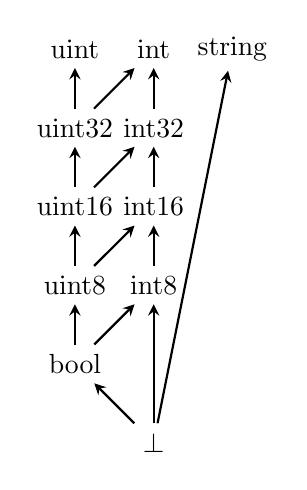
\begin{tikzpicture}
  \tikzstyle{EdgeStyle}=[->,>=stealth,thick]
  % nodes
  \node (UINT)                     {$\mycode{uint}$};
  \node (INT)    [right of=UINT]   {$\mycode{int}$};
  \node (STRING) [right of=INT]    {$\mycode{string}$};
  \node (UINT32) [below of=UINT]   {$\mycode{uint32}$};
  \node (INT32)  [right of=UINT32] {$\mycode{int32}$};
  \node (UINT16) [below of=UINT32] {$\mycode{uint16}$};
  \node (INT16)  [right of=UINT16] {$\mycode{int16}$};
  \node (UINT8)  [below of=UINT16] {$\mycode{uint8}$};
  \node (INT8)   [right of=UINT8]  {$\mycode{int8}$};
  \node (BOOL)   [below of=UINT8]  {$\mycode{bool}$};
  \node (BOT)    [below of=BOOL, below of=INT8]   {$\bot$};
  % edges
  \draw[EdgeStyle] (BOT) to node {} (BOOL);
  \draw[EdgeStyle] (BOT) to node {} (STRING);
  \draw[EdgeStyle] (BOT) to node {} (INT8);
  \draw[EdgeStyle] (BOOL) to node {} (UINT8);
  \draw[EdgeStyle] (BOOL) to node {} (INT8);
  \draw[EdgeStyle] (INT8) to node {} (INT16);
  \draw[EdgeStyle] (UINT8) to node {} (UINT16);
  \draw[EdgeStyle] (INT16) to node {} (INT32);
  \draw[EdgeStyle] (UINT16) to node {} (UINT32);
  \draw[EdgeStyle] (INT32) to node {} (INT);
  \draw[EdgeStyle] (UINT32) to node {} (UINT);
  \draw[EdgeStyle] (UINT8) to node {} (INT16);
  \draw[EdgeStyle] (UINT16) to node {} (INT32);
  \draw[EdgeStyle] (UINT32) to node {} (INT);
\end{tikzpicture}
\]

\subsubsection{Security types}
Data in SecreC is classified into the public and private domains. Hence, we use
\mycode{public} and \mycode{private} security classes to denote data
accordingly. These security classes can also be modeled after \cite{DENNING76}
to form a lattice. We denote the security classes using the meta-variable
$\tau$:
\[ \tau ::= \mycode{public}\ |\ \mycode{private}. \]

In addition, we define the binary $\oplus$ operator which is similar to the
$\oplus$ operator in \cite{DENNING76}. It is used in the static checking rules
in Subsection \ref{sec:checking:typing:expressions} to infer security types for
results of certain kinds of expressions. Although both return identical results
for security types, the latter is a total binary operation on the set of
security classes $\tau$ while on the other hand our $\oplus$ operator is a
binary operation on security types. Currently, we define the exact domain of
$\oplus$ only to include security classes:
\[
  \oplus : \tau \times \tau -> \tau
\]\[
\tau_1 \oplus \tau_2 = \begin{cases}
    \mycode{public}  &
      \text{if $\tau_1 = \mycode{public}$ and $\tau_2 = \mycode{public}$} \\
    \mycode{private} &
      \text{if $\tau_1 = \mycode{private}$ or $\tau_2 = \mycode{private}$}. \\
  \end{cases}
\]

The relation $->$ between security types defines the allowed direction of data
flow. For our security types, only the following hold:
\begin{align*}
  \mycode{private} & -> \mycode{private} \\
  \mycode{public}  & -> \mycode{public} \\
  \mycode{public}  & -> \mycode{private}
\end{align*}
meaning that data can flow in its own domain, and public data can flow into the
private domain.

\subsubsection{Dimensionality types}

Most of the data in SecreC can be multi-dimensional, and for that reason all
data types are supplied with dimensionality type. Scalar values are considered
to be 0-dimensional, vectors are 1-dimensional, matrices 2-dimensional, etc.
Formally dimensionality type is non-negative integer, and is denoted by either
$n$ or $m$.

In order to allow implicit conversions from scalar values to higher-dimensional
arrays, where context allows, we define partial ordering on dimensionalities.
We define that $0 \sqsubseteq n$ and $n \sqsubseteq n$ for every dimensionality
$n$.  Operator $n \sqcup m$ is defined as least upper bound of set $\left\{ n,
m \right\}$, if it exists. Intuition behind the ordering $n \sqsubseteq m$ is
that $n$-dimensional array is allowed to be converted into $m$-dimensional
array, and both $n$ and $m$ are allowed to be converted to $n \sqcup m$
dimensional array. The conversion may still fail at run-time if it turns out
that shapes of the arrays mismatch, and for that reason we will later define
similar ordering on shapes.

Because we can use previous ordering on lattice only if the context allows, for
example arithmetic operators, and not in all cases, we need to also define flat
ordering for dimensionalities. The second lattice is flat, and $n \preceq m$
iff $n = m$, and $\bot \preceq n$ for every $n$ and $m$. The partial ordering
relation also defines join $\curlyvee$ and meet $\curlywedge$ if they exist. This might
seem redundant to rename equality on non-negative numbers in such way, but
later we overload the $\preceq$ relation for all data types.

\subsection{The poset of data types}

As previously mentioned it's easy to construct Cartesian product from
fundamental data type, security type and dimensionality type partially ordered
sets, but it's complicated by the fact that we are dealing with two different
orderings depending on the context. For that reason we need to define two
different orderings for the data types as well.  In both cases we use $\bot$ to
mean product with all components are bottom as it's always clear from context
which poset it belongs to.

For contexts wherein scalar can be converted into higher dimensional array, we
use the regular ordering on dimensionalities. We say that $\alpha_1 \sqsubseteq
\alpha_2$ iff $\tau_1 \to \tau_2$,  $\delta_1 \sqsubseteq \delta_2$, and $n_1
\sqsubseteq n_2$, for every data type $\alpha_1 = \left( \tau_1, \delta_1, n_1
\right)$ and $\alpha_1 = \left( \tau_1, \delta_1, n_1 \right)$. We use $\sqcup$
for join and $\sqcap$ for meet.

For contexts that forbid scalar-to-array conversions we use flat ordering of
dimensionalities. This is to say that $\alpha_1 \preceq \alpha_2$ iff $\tau_1
\to \tau_2$,  $\delta_1 \sqsubseteq \delta_2$, and $n_1 \preceq n_2$, for every
data type $\alpha_1 = \left( \tau_1, \delta_1, n_1 \right)$ and $\alpha_1 =
\left( \tau_1, \delta_1, n_1 \right)$. We use $\curlyvee$ for join and
$\curlywedge$ for meet.



\subsection{Regular types}

The lower layer of the type system for SecreC defines properties for values and
variables in the language itself. Namely, each constant and expression, as well
as each defined variable and procedure in any valid SecreC program has a type
from the lower layer of this type system used for static checking.

An abstract type, denoted by the meta-variable $\rho$, is one of the following:
\begin{itemize}
  \item
    type $\mycode{void}$, also know as the \textit{unit type}, denotes data
    holding no information, i.e., allows only one possible value. It is not
    possible in SecreC to define variables of type \mycode{void}, or to work on
    values of type \mycode{void}. However, the return type of procedures may be
    defined to be \mycode{void}. In the latter case the procedure does not
    return a value, and such a procedure call can not be used as a
    subexpression, but only as a separate expression statement.

  \item data type $\alpha$ denoting the type of data held as values.

  \item  a variable type $\alpha\ var$ denoting the type of variables holding
    values of data type $\alpha$, i.e., the abstract data type of the
    \textit{l-value} for such variables\footnote{The primary reason for
    specifying a separate variable data type is for future purposes when
    support for references will be added to SecreC.}.

  \item a procedure type $\left(\alpha_1 \times \cdots \times \alpha_n\right)
    -> \alpha$ denoting procedures taking $n$ parameters (values) of types
    $\alpha_1,\cdots,\alpha_n$ and returning a value of type $\alpha$,

  \item a procedure type $\left(\alpha_1 \times \cdots \times \alpha_n\right) ->
    ()$ denoting procedures taking $n$ parameters (values) of types
    $\alpha_1,\cdots,\alpha_n$ and returning no value.

Formally:
\[
  \rho ::= \mycode{void}\ |\ \alpha\ |\ \alpha\ var\ |\  \left(\alpha_1 \times \cdots \times \alpha_n\right) -> \alpha\ |\ \left(\alpha_1 \times \cdots \times \alpha_n\right) -> ().
\]

\end{itemize}


\subsection{Statement types}
The middle layer of the type system for static checking deals with statements.
All statements in SecreC programs are contained in procedure bodies. Some
statements, like \mycode{if}-statements, loop constructs and compound
statements (statement blocks) may also contain other statements. For this
reason, we first define four properties for statements:
\begin{itemize}
\item $fallthru$ - the execution of the statement may end without reaching a
\mycode{return}, \mycode{break} or \mycode{continue} statement,
\item $return$ - the execution of the statement may end because of reaching a
\mycode{return} statement,
\item $break$ - the execution of the statement may end because of reaching a
\mycode{break} statement,
\item $continue$ - the execution of the statement may end because of reaching a
\mycode{continue} statement.
\end{itemize}

The type of a specific statement is determined by the set of properties that
hold for that statement. We denote the set of statement types with the
meta-variable $\Gamma_S$:
\[
\Gamma_S \in \mathcal{P}\!\left(\left\{ fallthru, return, break, continue \right\}\right).
\]

\subsection{Program types}
The higher layer of the type system for static checking deals with whole
programs. In this higher layer of the type system we denote the types of
programs with the meta-variable $\Gamma_P$. Currently, we are only interested
in whether a program is well-typed or not. Therefore, we only allow valid
programs to by typeable:
\[
\Gamma_P \in \left\{prog\right\}
\]
where $prog$ is the type of all well-typed programs.

\section{Typing rules}\label{sec:checking:typing}

Before presenting individual typing rules, we start by defining mangled
identifiers and a type environment, and describe how procedure overloading is
handled. The typing rules used for static checking are written as inference
rules with a syntax similar to \cite{VSI96} which has served as a basis for
inspiration.

\subsection{Identifiers and procedure overloading}\label{sec:checking:typing:identifiers}
In addition to identifiers $\operatorname{id}_S$ returned by the scanner (i.e.
  \bnfM{IDENTIFIER} tokens in Chapter \ref{sec:grammar}), we define the
entire set of identifiers $\operatorname{id}$ also to include \textit{mangled}
identifiers from a set $\operatorname{id}_M$ and a special identifier
\mycode{thisproc}. A mangled identifier for a procedure contains the name of
the procedure and information about the data types of its parameters. Mangled
identifiers are used to emulate procedure overloading. The special identifier
\mycode{thisproc} is used to denote the type of the procedure being
processed\footnote{Note that additional special identifiers may also be added
to the set of identifiers for the purpose of providing context-sensitive
information for inference rules defined in this chapter and also in the
semantics.}. The concrete set of elements in $\operatorname{id}_M$ as well
as the special identifier \mycode{thisproc} are implementation-specific,
but they are both required to be distinct from all possible identifiers
returned by the scanner, and distinct from each other. Hence, the whole set
of identifiers $\operatorname{id}$ can be formalized as

\[
\operatorname{id} = \operatorname{id}_S \uplus \operatorname{id}_M \uplus \{\mycode{thisproc}\}.
\]

For procedure overloading, we define a bijective function $\mathcal{M}$ for
procedure name mangling, which takes an identifier as returned by the scanner
and the list of data types of the procedure parameters, and returns a mangled
identifier:
\[
\mathcal{M} : \operatorname{id}_S \times \left(\alpha_1 \times \ldots \times \alpha_n \right) \rightarrow \operatorname{id}_M.
\]

The procedure overloading mechanism in this paper
allows several procedures with the same name to be present in SecreC programs.
Namely, for each two procedures with the same name, they must either take a
different number of parameters, or if they both take $n$ parameters then the
data type of the $i$\textsuperscript{th} parameter must differ, and
$i\in\{1\ldots n\}$.

In addition to overloading we support subtype polymorphism.  This is a
reasonable way to solve the ambiguity introduced by \cite{SECREC} which also
allows overloading on security types in the context where the security types of
the arguments can implicitly change.

\subsection{Type environment}\label{sec:checking:typing:environment}

According to the SecreC grammar in Chapter \ref{sec:grammar}, there are only
three distinct places where lookup or checking for the type for identifiers is
necessary: when assigning to variables in \bnfNT{assignment\_expression}, when
reading a variables in \bnfNT{primary\_expression}, and when calling
procedures in \bnfNT{postfix\_expression}. Every identifier typed by the
programmer, should only either refer to a variable, or to one or more
procedures.

According to the scoping rules formally defined later, for all identifiers $i$,
a definition of procedure $i$ irreversibly hides any previous definitions of
global variables $i$. A definition of global variable $i$ \textit{shadows} all
previous definitions of $i$, including the definitions of procedures $i$.
However, when defining another procedure $i$, any previous procedure
definitions are again \textit{un-shadowed} while the global variable definition
of $i$ is hidden. Similar rules are set for procedure parameters and local
variable definitions, which also hide all previous definitions for their scope.

Let $\gamma$ be a type environment, a partial function from the set of all
identifiers to the set of types
\[
\gamma: \operatorname{id} \hookrightarrow \rho \uplus \left\{A\ \mycode{proc}\ |\ A \subseteq A^0 \cup A^1 \cup \dots \right\},
\]
where $A\ \mycode{proc}$ denotes that the identifier given to $\gamma$ points
to some procedure defined on arguments of types in set $A$. The rationale
behind this is that when in some scope the last definition of the identifier
$i\in\operatorname{id}_S$ is a procedure definition, i.e., when
$\gamma\!\left(i\right)=A\ \mycode{proc}$ for the type environment $\gamma$ of
that scope, then $\gamma$ also returns the full type of the procedure
(including the security types of the parameters and the return type) when given
some mangled identifier of the procedure. Set of all valid argument types is
defined as follows:
\[
\begin{array}{ll}
  A^{0} &= \left\{ () \right\} \\
  A^{n+1} &= \left\{ (\alpha, \alpha_1, \dots, \alpha_n)\ |\ \left( \alpha_1, \dots, \alpha_n \right) \in A^n, \text{$\alpha$ is a data type} \right\} \\
\end{array}
\]

Updating a type environment $\gamma$ with a definition of $x$ having type $t$,
where $t \in \rho \uplus \left\{\mycode{proc}\right\}$, is denoted by
$\gamma\!\left[ x |-> t \right]$ and defined by the following equation:
\[ \gamma\!\left[ x |-> t \right]\left(x'\right) = \left\{\begin{array}{ll}
    t                  & \quad \text{if $x' = x$}\\
    \gamma\!\left(x'\right) & \quad \text{if $x' \not = x$}.
  \end{array}\right.
\]
Updating the type environment is what hides or shadows (or un-shadows) any
previous definitions of the given identifier. When defining a new procedure
denoted by the identifier $i$, one needs to update the type environment twice:
first to point the identifier $i$ to \mycode{proc}, and secondly to point the
mangled $i$ to the actual type of the procedure.

\subsection{Checking expressions}\label{sec:checking:typing:expressions}

In this section, we denote expressions with $e$, variables with $x$, procedure
names with $f$ and values with the meta-variable $v$.

The $\eta$EConst rule defines the type for explicit values typed by the
programmer such as decimal or string literals and keywords \mycode{true} and
\mycode{false} which correspond to boolean constants:
\[ \inference[$\eta$EConst]{
  \operatorname{validLiteral}(v)
}{
  \gamma |- v : (\mycode{public}, \operatorname{datatype}(v), 0)
} \]
where function $\operatorname{datatype}\!\left(v\right)$ is the data type of
value or literal $v$, and the predicate $\operatorname{validLiteral}$ checks
whether the given literal is a valid string, integer, unsigned integer or
boolean literal. It's currently not possible to construct non-scalar literals,
we have found that it is rarely required with implicit conversion of scalars to
arrays.

For string literals the predicate $\operatorname{validLiteral}$
checks that there are no invalid or incomplete escape sequences in the string.
For integer and unsigned integer literals it checks whether the corresponding
decimal value fits into the corresponding 32-bit signed or unsigned integer
data type. The function
$\operatorname{datatype}$ is defined as follows:
\[
 \operatorname{datatype}\!\left(v\right) = \left\{\begin{array}{rll}
                                            \mycode{string} & \qquad\mbox{if $v$ is a string literal} \\
                                            \mycode{bool} & \qquad\mbox{if $v$ is \mycode{true} or \mycode{false}} \\
                                            \mycode{unsigned int} & \qquad\mbox{if $v$ is a integer literal} \\
                                            \mycode{int} & \qquad\mbox{if $v$ is an unsigned integer literal.}
                                           \end{array}\right.
\]

For variables or functions symbols appearing as \textit{r-values}, the
$\eta$ERValue and $\eta$ERProc can be used, which infers the type of the value
held by some symbol.
\[
\inference[$\eta$ERValue]{
  \gamma(x) = \alpha\ var
}
{
  \gamma |- x : \alpha
}
\]
\[
\inference[$\eta$ERProc]{
  \gamma(f) = A\ \mycode{proc}
}
{
  \gamma |- f :  A\ \mycode{proc}
}
\]

According to $\eta$EBinary, the data type of binary expressions depends on the
types of the operands. The subexpressions are required to
have fundamental data types, and the security type of the binary expression is
the safest security type of the subexpressions. The partial function
$\operatorname{BOT}_\anyop$ returns the data type for all binary operations
$\anyop \in \left\{\mycode{||}, \mycode{&&}, \mycode{==}, \mycode{!=},
\mycode{<}, \mycode{<=}, \mycode{>=}, \mycode{>}, \mycode{+}, \mycode{-},
\mycode{*}, \mycode{/}, \mycode{\%}\right\}$ and is tabulated in Appendix
\ref{appendix:binary}. Note, that for some operators both the allowed security
types and data types differ from \cite{SECREC}. Dimensionality of resulting
expression is defined by least upper bound of the subexpression dimensionalities.
This allows for scalar value to appear in expressions where it can be implicitly
converted into higer dimensional array.
\[ \inference[$\eta$EBinary]
{
  \gamma |- e_1 : \left(\tau_1, \delta_1, n_1\right) \\
  \gamma |- e_2 : \left(\tau_2, \delta_2, n_2\right) \\
  \tau = \tau_1 \oplus \tau_2&
  \delta = \operatorname{BOT}_{\anyop}(\delta_1, \delta_2)&
  n = n_1 \sqcup n_2
}{
  \gamma |- e_1 \circledast e_2 : \left(\tau, \delta, n\right)
} \]

% ETernary
For ternary expressions, the rule $\eta$ETernary requires the conditional
expression to be public boolean to do the branching. The data types of both
branches of the ternary expression are required to be fundamental data types
and equal, and the security type of the ternary expression depends on the
security types of the branches. Unlike binary expression we restrict
dimensionalities of branches to be equal and impose that conditional expression
is either scalar or its dimensionality is same as that of resulting expression.
Those restrictions are in place so that the ternary expression operates
point-wise and has to evaluate both arguments only if the conditional
expression is non-scalar.
\[ \inference[$\eta$ETernary]
{
    \gamma |- e : \left(\mycode{public}, \mycode{bool}, n_0\right) \\
    \gamma |- e_1 : \left(\tau_1, \delta_1, n\right),\  \gamma |- e_2 : \left(\tau_2, \delta_2, n \right) \\
    \tau = \tau_1 \oplus \tau_2,\ \delta = \delta_1 \sqcup \delta_2,\ n_0 \sqsubseteq n \\
}{
  \gamma |- e\ \mycode{?}\ e_1\ \mycode{:}\ e_2\ :\ \left(\tau, \delta, n\right)
} \]

For a ternary expression a simple optimization is to calculate one branch,
depending on the value of the conditional. Since directing the control flow on
\mycode{private} conditions causes side-channel information leaks in Sharemind,
we require the ternary conditional always to be \mycode{public} to avoid
ambiguity which would arise from different semantic rules depending on the
security type of the conditional. Namely, it is in some cases possible to have
safe ternary expressions with \mycode{private} conditional expressions, but its
semantics would require both branches to be calculated regardless of the value
of the conditional. For similar reason we restrict branches to have equal
dimensionalities. If one branch is scalar and other is not, we would need to
evaluate the non-scalar branch regardless of which value conditional takes in
order to shape non-scalar appropriately.

% EAssignOp
In rule $\eta$EAssignOp for regular assignment expressions, we just require the
variable we assign to (the l-value) to hold values of the same type as the
expression (r-value) we assign to it. In addition right hand side can be of
looser security type and is allowed to be scalar value even if left hand side
is not.
\[ \inference[$\eta$EAssignOp]
{
  \gamma(x) = \alpha\ \mathit{var} &
  \gamma |- e : \alpha' &
  \alpha' \sqsubseteq \alpha
}
{
  \gamma |- x\ \mycode{=}\ e : \alpha
} \]

% EAssignOp2
For arithmetic assignment expressions that perform calculations based on the
current value of the variable, $\eta$EAssignOp2 requires that the corresponding
binary arithmetic operation between the l-value and the r-value is typeable,
and that the variable being assigned to can hold the result of this operation.
\[ \inference[$\eta$EAssignOp2]
{
  \gamma(x) = \alpha\ \mathit{var} &
  \gamma |- x \circledast e : \alpha' &
  \alpha' \preceq \alpha
}
{
  \gamma |- x\  \circledast \mycode{=}\ e : \alpha
} \]

% ENeg ENot
Typing rules for unary operators only require certain data types for its
operands, namely the $\eta$ENot rule for logical negation and the $\eta$ENeg
for numerical negation require their operands to be of data types \mycode{bool}
or \mycode{int} respectively.
\[\begin{array}{c}
\inference[$\eta$ENot]{\gamma |- e : (\tau, \mycode{bool}, n)}{\gamma |- \mycode{!}e : (\tau, \mycode{bool}, n)} \\[2em]

\inference[$\eta$ENeg]{
  \gamma |- e : (\tau, \delta, n) \\
  \delta' = \min \left\{ \delta'\in\mathtt{Signed}\ |\ \delta \sqsubseteq \delta' \right\}
}{
  \gamma |- \mycode{-}e : (\tau, \delta', n)
}
\end{array} \]
As unary negation is only defined on signed integer types we define set
$\mathtt{Signed} = \left\{ \mycode{int8}, \mycode{int16}, \mycode{int32}, \mycode{int} \right\}$ to enumerate all
types negation can be called directly called on. In the inference rule we
compute the smallest type we can cast the argument to, and use that as
resulting type. Type checking may fail if the unique minimal element does not
exist.

% EDeclassify
The $\eta$EDeclassify rule is used to convert \mycode{private} data into
\mycode{public} data. Without this rule it is impossible to transfer any
information from \mycode{private} values to \mycode{public} variables or
output. By requiring the argument to be of \mycode{private} security type,
expressions like \mycode{declassify(declassify(e))} are not possible.
\[
\inference[$\eta$EDeclassify]{\gamma |- e : (\mycode{private}, \delta, n)}{\gamma |- \mycode{declassify(e)} : (\mycode{public}, \delta, n)}
\]

% EProcCall
For procedure calls, the $\eta$EProcCall rule first checks whether the
procedure identifier $f$ is of type \mycode{proc} according to the type
environment, that all the given arguments type-check properly, and have value
types. After this, it must be checked whether the mangled identifier $f$ is in
the type environment and whether the security types for the arguments can
satisfy the security types for the procedure parameters. These checks are part
of the procedure overloading mechanism. The result type for the procedure call
can also be calculated from the procedure type returned from the type
environment by its mangled identifier.
\[ \inference[$\eta$EProcCall]{
  \gamma |- f : A\ \mycode{proc}\\
  \gamma |- e_1 : \alpha_1, \cdots, \gamma |- e_m : \alpha_m \\
  A_f = \left\{ (\underline{\alpha}_1, \dots, \underline{\alpha}_m) \in A\ |\ \alpha_i \preceq \underline{\alpha}_i, 1 \le i \le m \right\}\\
  (\alpha'_1, \dots, \alpha'_m) = \min A_f \\
  \gamma |- \mathcal{M}(f, \alpha'_1, \cdots, \alpha'_m)
  : \left( \alpha'_1 \times \cdots \times \alpha'_m \right)  \to \rho \\
}{
\gamma |- f\mycode{(}e_1\mycode{,}\cdots\mycode{,}e_m\mycode{)} : \rho
}
\]

% EIndex
To express indexing of $n$-dimensional array we use $1 \leq \sigma(1) < \ldots
< \sigma(k) \leq n$ to denote those $k$ indices that are slices. Now, for all
$i$ in $\{1, \ldots, n\}$, if there is $j$ in $\{1,\ldots,k\}$, such that $i =
\sigma(j)$, then $\iota_i \equiv e_i : e'_j$, otherwise $\iota_i \equiv e_i$.
The rule $\eta$EIndex imposes that all $n$ indices are given and that all of
the indices are public integers. We see that dimensionality of resulting
expression can be computed by simply counting all the slices.
\[
\inference[$\eta$EIndex]
{
  \gamma |- e : \left( \tau, \delta, n \right) \\
  \gamma |- e_1 : \alpha_1,\ \ldots,\ \gamma |- e_n : \alpha_n \\
  \gamma |- e'_1 : \alpha'_1,\ \ldots,\ \gamma |- e'_k : \alpha'_k \\
  \alpha_i \sqsubseteq (\mycode{public}, \mycode{int}, 0), 1 \le i \le n \\
  \alpha'_j \sqsubseteq (\mycode{public}, \mycode{int}, 0), 1 \le j \le k
}
{
  \gamma |- e \mycode{[} \iota_1, \ldots, \iota_n \mycode{]} : \left(\tau, \delta, k\right)
}
\]

% TODO syntactic sugar should be explained elsewhere?
Syntactically we allow, in addition to regular slices \mycode{i:j}, for either
of the slice bounds to be missing. Missing lower bound is always interpreted as
constant $0$, and missing upper bound of $k$-th dimension is interpreted as
value that equals to the size of $k$-th dimension.

% EAssignArray
For left hand side indexing, the $\eta$AssignArray rule is similarly to regular
indexing rule, but in addition we have to check that the value of right hand
side expression can be assigned to $x$ types. This means that we allow for
right hand side to have laxer security type, right hand side may be sub-type of
left hand side and scalar may appear in right hand side. Ofcourse as with
previous rule we have to check that the indices can be casted to public integer
scalars.
\[ \inference[$\eta$EAssignArray]
{
  \gamma(x) = \alpha\ \mathit{var}  &
  \gamma |- e : \alpha' & \alpha' \sqsubseteq \alpha \\
  \gamma |- e_1 : \alpha_1,\ \ldots,\ \gamma |- e_n : \alpha_n \\
  \gamma |- e'_1 : \alpha'_1,\ \ldots,\ \gamma |- e'_k : \alpha'_k \\
  \alpha_i \sqsubseteq (\mycode{public}, \mycode{int}, 0), 1 \le i \le n \\
  \alpha'_j \sqsubseteq (\mycode{public}, \mycode{int}, 0), 1 \le j \le k
}
{
  \gamma |- x \mycode{[} \iota_1, \ldots, \iota_n \mycode{]}\ \mycode{=}\ e : \alpha
} \]

% EAssignArrayOp
Array assignment with operator is similar to $\eta$AssignOp2 rule.
\[ \inference[$\eta$EAssignArrayOp]
{
\gamma(x) = \alpha\ \mathit{var} \\
  \gamma |-  x \mycode{[} \iota_1, \ldots, \iota_n \mycode{]} \circledast e : \alpha' \\
  \alpha' \preceq \alpha
}
{
  \gamma |- x \mycode{[} \iota_1, \ldots, \iota_n \mycode{]}\ \circledast \mycode{=}\ e : \alpha
} \]

% EShape, ESize
Two similar rules $\eta$EShape and $\eta$ESize  can be used to query the shape
and size of arrays, they return either public vector of integers or public
integer respecively. The rules don't impose any restrictions on the
type of the arguments.
\[ \inference[$\eta$EShape]
{
  \gamma |- e : \alpha
}
{
  \gamma |- \mycode{shape(} e \mycode{)} : \left(\mycode{public}, \mycode{int}, 1\right)
} \]
\[ \inference[$\eta$ESize]
{
  \gamma |- e : \alpha
}
{
  \gamma |- \mycode{size(} e \mycode{)} : \left(\mycode{public}, \mycode{int}, 0\right)
} \]
% EReshape

The $\eta$EReshape rule allows to construct new arrays with different shape and
dimensionality, but with same data. We don't impose any restrictions on first
argument, but all following arguments have to be public integer scalars.
Resulting expression has same security type and same data type as first
argument, but the new dimensionality.
\[ \inference[$\eta$EReshape]
{
  \gamma |- e : \left(\tau, \delta, n\right) \\
  \gamma |- e_1 : \left(\mycode{public}, \delta_1, 0\right) & \delta_1 \sqsubseteq \mycode{int} \\
  \vdots \\
  \gamma |- e_k : \left(\mycode{public}, \delta_k, 0\right) & \delta_k \sqsubseteq \mycode{int}     }
{
  \gamma |- \mycode{reshape(} e , e_1, \ldots, e_k \mycode{)} : \left(\tau, \delta, k\right)
} \]

% ECat
For generic concatenation of arrays we use rule $\eta$ECat. The expression has
three arguments, first two are equal dimensional arrays and third is integer
literal that denotes the dimension along which we glue the arrays together.
Resulting array has same data type and dimensionality as first two and stricter
of the security types.
\[ \inference[$\eta$ECat]
{
  \gamma |- e_0 : \alpha_0 &
  \gamma |- e_1 : \alpha_1 &
  0 \leq k < n
} 
{
  \gamma |- \mycode{cat(} e_0 , e_1, k \mycode{)} : \alpha_0 \curlyvee \alpha_1
} \]


In the following sections, let the predicate
$\operatorname{goodexpr}\!\left(\gamma, e\right)$ check whether the expression
$e$ properly type-checks in the type environment $\gamma$, i.e., that there
exists some $\rho$ so that $\gamma |- e : \rho$.

\subsection{Checking statements}\label{sec:checking:typing:statements}

Statements are checked in a sequential manner -- one after the other -- using
the meta-variable $S$ to denote any following statements. For some rules,
however, no following statements are allowed. The type for any set of
sequential statements denotes the set of possible results for executing these
statements. For example, for an \mycode{if} statement where one branch always
ends with a \mycode{return} and the other branch always ends with a
\mycode{break}, then the type of that \mycode{if} statement would be
$\left\{break, return\right\}$, and static checking does not allow any
statements to directly follow that \mycode{if} statement.

The static checking rules $\eta$SBreak for \mycode{break} statements,
$\eta$SContinue for \mycode{continue} statements, $\eta$SReturn and
$\eta$SReturnVoid for \mycode{return} statements don't allow any statements to
follow. This forces the programmer not to write any unreachable code directly
after these statements. For \mycode{return} statements, an additional check for
the return type is done. The type of the empty statement according to
$\eta$SEmpty is $\emptyset$.
\[ \begin{array}{c}
\inference[$\eta$SBreak]{}{\gamma |- \mycode{break;} : \left\{ break \right\} } \\[2em]
\inference[$\eta$SContinue]{}{\gamma |- \mycode{continue;} : \left\{ continue\right\} } \\[2em]
\inference[$\eta$SEmpty]{}{\gamma |- \varepsilon\mycode{;} : \emptyset } \\[2em]
\inference[$\eta$SReturnVoid]{
  \gamma(\mycode{thisproc}) = (\alpha_1\times\dots\times\alpha_n)\to()
}{
  \gamma |- \mycode{return;} : \left\{ return \right\}
} \\[2em]
\inference[$\eta$SReturn]{
  \gamma |- e : \alpha' \\
  \gamma(\mycode{thisproc}) = (\alpha_1\times\dots\times\alpha_m)\to\alpha \\
  \alpha' \preceq \alpha \\
}{
  \gamma |- \mycode{return}\ e \mycode{;} : \left\{ return \right\}
}
\end{array}\]


For compound statements, three different cases have to be considered. The first
two cases deal with local variable definitions followed by statements in the
type environment updated with the new variable type. Each local variable
definition can be viewed as a definition of a new scope for variables.
Therefore, the rules $\eta$SCompoundVarDef and $\eta$SCompoundVarDefInit only
allow variable definitions to be followed by at least one non-empty statement.
The opposite case -- to define the variable and then just discard it together
with the scope -- would make no sense, since one could instead just use an
expression statement. In the $\eta$SCompoundVarDefInit rule, the type of the
initializer expression is also checked to correspond to the type of the
variable being defined.
\[\begin{array}{c}
\inference[$\eta$SCompoundVarDef]{
  \gamma |- e_1 : \left( \mycode{public}, \delta_1, 0 \right), \delta_1 \sqsubseteq \mycode{int} \\
  \vdots \\
  \gamma |- e_n : \left( \mycode{public}, \delta_n, 0 \right), \delta_n \sqsubseteq \mycode{int}\\
  \gamma[x \mapsto (\tau, \delta, n)\ \mathit{var}] |- S : \Gamma_S \\
  \Gamma_S \neq \emptyset
}{
  \gamma |- \tau\ \delta\ \mycode{[[}n\mycode{]]}\ x\mycode{[} e_1 \mycode{,} \ldots \mycode{,} e_n \mycode{];} S : \Gamma_S
} \\[2em]
\inference[$\eta$SCompoundVarDefInit]{
  \gamma |- e_1 : \left( \mycode{public}, \delta_1, 0 \right), \delta_1 \sqsubseteq \mycode{int} \\
  \vdots \\
  \gamma |- e_n : \left( \mycode{public}, \delta_n, 0 \right), \delta_n \sqsubseteq \mycode{int}\\
  \gamma |- e : \left( \tau', \delta', n' \right) \\
  \gamma[x \mapsto (\tau, \delta, n)\ \mathit{var}] |- S : \Gamma_S \\
  \Gamma_S \neq \emptyset \\
  \tau' \to \tau,\ \delta' \sqsubseteq \delta,\ n' \sqsubseteq n
}{
  \gamma |- \tau\ \delta\ \mycode{[[}n\mycode{]]}\ x\mycode{[} e_1 \mycode{,} \ldots \mycode{,} e_n  \mycode{]=}\ e\mycode{;} S : \Gamma_S
}
\end{array}\]

For conciseness we allow some syntactic sugar. Variable is considered to be
scalar if the dimensionality annotation $\mycode{[[}n\mycode{]]}$ is omitted.
If shape $\mycode{[} e_1 \mycode{,} \ldots \mycode{,} e_n  \mycode{]}$ is
missing we take all dimensions to be empty.

The third case considers some regular statement following the rest of the
compound statement. The type of the regular statement is expected to include
$fallthru$, otherwise the rest of the statements would be unreachable code. The
$\eta$SCompound rule also does not allow empty statements (with statement type
$\emptyset$) to precede any other statements.
\[ \inference[$\eta$SCompound]{
  \gamma |- S : \Gamma_S & fallthru \in \Gamma_S & \gamma |- S' : \Gamma'_S
}{
  \gamma |- S\mycode{;}S' : \left( \Gamma_S \setminus \left\{ fallthru \right\} \right) \cup \Gamma'_S
} \]

For expression statements, it is only checked whether the expression is valid.
The type for expression statements is defined just to be $\left\{ fallthru
\right\}$:
\[ \inference[$\eta$SExpr]{
  \operatorname{goodexp}\left( \gamma, e \right)
}{
  \gamma |- e : \left\{ fallthru \right\}
} \]

All guards (conditional expressions) in statements are checked to be of public
boolean scalar type. The security type is enforced to be \mycode{public} to
prevent information leakage from control flow in the underlying virtual
machine. Let the predicate $\operatorname{goodguard}\!\left(\gamma, e\right)$
check whether the type of the given expression $e$ is $\left(\mycode{public},
\mycode{bool}\ 0\right)$ in the given type environment $\gamma$, i.e., that
$\gamma |- e : \left(\mycode{public}, \mycode{bool}\ 0\right)$ holds.

The type of \mycode{if} statements is determined by the types of its branches.
First, it is required that the branches are not empty. If one or both branches
are found of type $\emptyset$, the statement should be refactored by the
programmer for code clarity. For \mycode{if} statements without an
\mycode{else} branch, it is still possible that the statements in the first
branch are not executed, therefore the type of the \mycode{if} statement must
also contain $fallthru$. For \mycode{if} statements with both branches, the
type of the whole \mycode{if} statement is just the set union of the types of
its two branches.
\[\begin{array}{c}
\inference[$\eta$SIf]{
  \goodguard\left( \gamma, e \right) &
    \gamma |- S : \Gamma_S &
    \Gamma_S \neq \emptyset
}{
  \gamma |- \mycode{if(}e\mycode{)}\ S : \Gamma_S \cup \left\{ fallthru \right\}
} \\[2em]
\inference[$\eta$SIfElse]{
  \goodguard\left( \gamma, e \right) &
    \gamma |- S : \Gamma_S &
    \Gamma_S \neq \emptyset &
    \gamma |- S' : \Gamma'_S &
    \Gamma'_S \neq \emptyset
}{
  \gamma |- \mycode{if(}e\mycode{)}\ S\ \mycode{else}\ S' : \Gamma_S \cup \Gamma'_S
}
\end{array} \]

To further enforce a good programming style, the types of the bodies of all
loops in SecreC are required either to contain $fallthru$ or $continue$ or be
$\emptyset$, meaning that it might be possible for the loop to do more than one
iteration. Otherwise, the loop can be substituted with acyclic code. The bodies
of the loops also filter out $break$ and $continue$ from the type of the loop
body. Hence, in principle, the type of a loop is $\left\{fallthru,
return\right\}$ if the type of the body of the loop contains $return$, and
$\left\{fallthru\right\}$ otherwise.

Let $\Gamma_B$ denote the type of the loop body for all static checking rules
for loops, and $\Gamma_L$ denote the set $\left(\Gamma_B \setminus \left\{
break , continue \right\}\right) \cup \left\{ fallthru \right\}$, which is
the type of the entire loop. Let the predicate
$\operatorname{goodbody}\!\left(\Gamma_B\right)$ check whether $\Gamma_B
= \emptyset$ or that $\Gamma_B \cap \left\{ continue, fallthru \right\}
  \not = \emptyset$ holds for the given $\Gamma_B$.

The static checking rules for \mycode{while} and \mycode{do}-\mycode{while}
loops are identical:
\[\begin{array}{c}
\inference[$\eta$SWhile]
{ % Joone peal:
  \operatorname{goodguard}\!\left(\gamma, e\right)
  & \gamma |- S : \Gamma_B
  & \operatorname{goodbody}\!\left(\Gamma_B\right)
}{ % Joone all:
  \gamma |- \mycode{while}\ \mycode{(}e\mycode{)}\ S : \Gamma_L
} \\[2em]
\inference[$\eta$SDoWhile]
{ % Joone peal:
  \operatorname{goodguard}\!\left(\gamma, e\right)
  & \gamma |- S : \Gamma_B
  & \operatorname{goodbody}\!\left(\Gamma_B\right)
}{ % Joone all:
  \gamma |- \mycode{do}\ S\ \mycode{while}\ \mycode{(}e\mycode{);} : \Gamma_L
}
\end{array} \]


% TODO
The most complex loop in SecreC is the \mycode{for} loop. Since all the three
expressions are optional, we would have to formulated a separate rule for each
such case, and have a total of eight rules. Luckily all cases are simple
alterations of most general one and we just explain them in text. If present,
the first and last expressions are only checked for validity. The second
expression is the loop guard, and is checked just like guards in other
statements. When the guard is omitted, the respective rules ensure, that the
type of the body of the loop contains either $break$ or $return$ to catch
trivial cases of non-terminating loops.
\[ \inference[$\eta$SFor]
{ % Joone peal:
  \operatorname{goodexpr}\!\left(\gamma, e\right) \\
  \operatorname{goodguard}\!\left(\gamma, e'\right) \\
  \operatorname{goodexpr}\!\left(\gamma, e''\right) \\
  \gamma |- S : \Gamma_B \\
  \operatorname{goodbody}\!\left(\Gamma_B\right)
}{ % Joone all:
  \gamma |- \mycode{for}\ \mycode{(}e\mycode{;}\ e'\mycode{;}\ e''\mycode{)}\ S : \Gamma_L
} \]

Like mentioned all other cases are similar to most general one. Namely, we
allow for any combination of the expressions to be missing, and in all cases we
just omit either the corresponding $\operatorname{goodexpr}$ or
$\operatorname{goodguard}$ checks. In all cases where guard is missing we check
if either $break$ or $return$ is in $\Gamma_B$ to avoid trivially looping
programs.

\subsection{Checking programs}\label{sec:checking:typing:programs}

Similarly to the techniques described in Subsection
\ref{sec:checking:typing:statements}, the static checking of programs is also
performed in a sequential manner -- on a definition-by-definition basis. This
is done by checking each global variable or procedure definition by itself and
then checking the rest of the program in a type environment updated with all
previous definitions. Checking starts with a predefined type environment
$\gamma_0$ which may also be empty, i.e., with an empty domain, meaning that
there are no predefined variables or procedures.

We denote the domain of a (partial) function $f$ by
$\operatorname{dom}\!\left(f\right)$, and use the meta-variable $P$ to denote
program fragments. 

For global variable definitions without initializer expressions we check that
subexpressions denoting shape of declared variable are public integers,
type environment $\gamma$ is updated with the variable being defined, and the
rest of the program is checked in the updated type environment:
\[ \inference[$\eta$VarDef]{
  \gamma |- e_1 : \left( \mycode{public}, \delta_1, 0 \right), \delta_1 \sqsubseteq \mycode{int} \\
  \vdots \\
  \gamma |- e_n : \left( \mycode{public}, \delta_n, 0 \right), \delta_n \sqsubseteq \mycode{int} \\
  \gamma[x \mapsto \left( \tau, \delta, n \right) \mathit{var}] |- P : \Gamma_P
}{
  \gamma |- \tau\ \delta\ \mycode{[[}n\mycode{]]}\ x\mycode{[} e_1 \mycode{,} \ldots \mycode{,} e_n  \mycode{];} P : \Gamma_P
} \]

Static checking of global variable definitions with initializer expressions is
performed as without initializer expressions, with the only exception, that the
initializer expression is first checked in the type environment before updating
it.
\[ \inference[$\eta$VarDefInit]{
  \gamma |- e_1 : \left( \mycode{public}, \delta_1, 0 \right), \delta_1 \sqsubseteq \mycode{int} \\
  \vdots \\
  \gamma |- e_n : \left( \mycode{public}, \delta_n, 0 \right), \delta_n \sqsubseteq \mycode{int} \\
  \gamma |- e : \left( \tau', \delta', n' \right) \\
  \tau' \to \tau,\ \delta' \sqsubseteq \delta,\ n' \sqsubseteq n \\
  \gamma[x \mapsto (\tau, \delta, n)\ \mathit{var}] |- P : \Gamma_P
}{
  \gamma |- \tau\ \delta\ \mycode{[[}n\mycode{]]}\ x\mycode{[} e_1 \mycode{,} \ldots \mycode{,} e_n  \mycode{]=}\ e\mycode{;} P : \Gamma_P
} \]

Similarly to local declarations by having intuitive default values we allow the
shape and dimensionality to be omitted in both cases. Declared values without
dimensionality annotation are scalars, and missing shape annotation means shape
with all dimension sizes of zero. We do not introduce rules for those cases, as
it's just syntactic sugar and transformation to general case can be performed
before static checking.

For procedure definitions, it is first verified that the type environment does
not already contain a procedure with the same signature (its mangled
identifier). Secondly, it is verified that no two names for the procedure
parameters are equal, ensuring that the parameters do not hide each other.
Thirdly, the body of the function is type-checked to verify its internal
structure and that it always returns a value of the correct type (or falls
through without returning in case the return type is \mycode{void}).  Finally,
the program following this definition is checked in the type environment
updated with this procedure.

An updated type environment is used for type-checking the procedure body. This
type environment is not only updated with the definition of the current
procedure (to allow recursion), but also with the procedure parameters. To
type-check all the return statements in the function body we also extend the
type environment using \mycode{thisproc} to point to the type of the enclosing
procedure. For procedures returning a value in rule $\eta$Procdef, the body of
the procedure must be of statement type $return$, while for \mycode{void}
procedures in rule $\eta$ProcdefVoid, the body of the procedure might also be
of type $fallthru$. An additional check ensures that a procedure named
\mycode{main} taking no parameters can only be of \mycode{void} return type.
\[\begin{array}{c}
\inference[$\eta$Procdef]{
  \mathcal{M}^f \notin \operatorname{dom}\left( \gamma \right) \\
    f \neq \mycode{main} \lor n > 0 \\
    \gamma_c |- S : \left\{ return \right\} \\
    \gamma' |- P : \Gamma_P
}{
  \gamma |- \alpha\ f\mycode{(} \alpha_1\ p_1 \mycode{,} \ldots \mycode{,}\ \alpha_n\ p_n\mycode{) \{}S\mycode{\}}\ P : \Gamma_P
} \\[2em]
\inference[$\eta$ProcdefVoid]{
  \mathcal{M}^f \notin \operatorname{dom}\left( \gamma \right) \\
    \gamma_c |- S : \Gamma_S \\
    \Gamma_S \subseteq \left\{ fallthru, return \right\} \\
    \gamma' |- P : \Gamma_P
}{
  \gamma |- \mycode{void}\ f\mycode{(} \alpha_1\ p_1 \mycode{,} \ldots \mycode{,}\ \alpha_n\ p_n\mycode{) \{}S\mycode{\}}\ P : \Gamma_P
}
\end{array} \]
where \[\begin{array}{rcl}
  \mathcal{M}^f & = & \mathcal{M}(f,\alpha_1,\ldots,\alpha_n) \\
    A           & = & 
      \left\{ (\alpha_1,\ldots,\alpha_n) \right\} \cup 
      \left\{ \overline{\alpha} \in A'\ |\ \gamma(f) = A'\ \mycode{proc} \right\} \\
    \gamma'     & = & \gamma[f \mapsto A\ \mycode{proc}]\left[ \mathcal{M}^f \mapsto \rho \right] \\
    \gamma_c    & = & \gamma'[\mycode{thisproc} \mapsto \rho]
                             [p_1 \mapsto \alpha_1]\dots[p_n \mapsto \alpha_n] \\
    \rho        & = & \begin{cases} 
       (\alpha_1\times\ldots\times\alpha_n)\to\alpha & \text{if Procdef} \\
       (\alpha_1\times\ldots\times\alpha_n)\to() & \text{if ProcdefVoid}. \\
    \end{cases}
\end{array}\]
\vspace{0.5cm}

After checking whether all the top-level definitions in the SecreC program are
correct, static checking verifies that a function called "main" taking no
parameters and returning no value exists:
\[ \inference[$\eta$ProgEnd]{
  \gamma(\mathcal{M}(\mycode{main}, ())) = ()\to()
}{
  \gamma |- \varepsilon : prog
} \]

\chapter{Natural semantics}\label{sec:semantics}

For the natural semantics (or big-step semantics), we use $->$ to denote
different transitions of state. Transitions for evaluating expressions are
denoted as $->_E$, transitions for evaluating defining variables and procedures
are denoted as $->_{DV}$ and $->_{DP}$ respectively, transitions for evaluating
statements and statement lists are denoted as $->_S$ and $->_{*}$ respectively,
and the transitions for evaluating the top level of the program are denoted by
$->$ only.

In this section, we first define representation of arrays and tools for
manipulating array indices, secondly we describe a more flexible way to handle
variables, and then continue to present evaluation rules for SecreC
expressions, variable definitions, statements, procedure definitions and the
program as a whole.

\section{Arrays}\label{sec:semantics:arrays}

Semantically all SecreC values are arbitrary-dimensional arrays of primitive
data.  As previously stated the dimensionality of arrays is known statically,
but sizes of each dimension, or in another words, shape of an array, is only
known at run-time. Thus at run-time we need to tie a tuple of integers $(d_1,
\ldots, d_n)$ with each $n$-dimensional array.

For static checking we defined ordering on dimensionalities, now we need to do
same for shapes aswell. For every shape $s$ we have that $() \sqsubseteq s$ and
$s \sqsubseteq s$. Operator $s_1 \sqcup s_2$ is defined as least upper bound of
set $\left\{ s_1, s_2 \right\}$. The upper bound operator is used for
calculating the shape of resulting array if scalar value need to be implicitly
converted to higher-dimensional array.

We represent $n$-dimensional values as partial functions from integer $n$-tuple
to the primitive base type:
\[
  \operatorname{val} : \underbrace{\mycode{int},\ldots,\mycode{int}}_{n} \hookrightarrow \sigma
\]
This aproach works on scalar values as per well known fact that $A$ is isomorphic to $() \to A$.

% TODO row major order
For every shape $s \equiv (d_1, \ldots, d_n)$ we define set of legal indices:
\[
  \mathcal{J}\!(s) = \{ (i_1, \ldots, i_n)\ |\ 0 \leq i_1 < d_1, \ldots, 0 \leq i_n < d_n \},
\]
and a class of bijective functions for ``flattening'' such sets:
\[
  \phi_{(d_1,\ldots,d_n)} : \mathcal{J}\!(d_1,\ldots,d_n) \to \mathcal{J}\!(d_1 d_2 \ldots d_n).
\]
The bijective function is not uniquely defined for a fixed shape, and for that
reason we fix one in so called ``column-major'' order:
\begin{align*}
  \phi_{(d_1,\ldots,d_n)}\!(i_1,\ldots,i_n) & = s_1 i_1 + s_2 i_2 + s_3 i_3 + \ldots + s_n i_n = \sum_{k = 1}^{n} s_k i_k,
\end{align*}
where $s_k = \prod_{i=1}^{k-1} d_i$ is the stride of $k$-th dimension. Using the inverse:
\begin{align*}
  \phi_{(d_1,\ldots,d_n)}^{-1}\!(x) & = (i_1, \ldots, i_n),\ \text{where} \\
                                i_1 & = x / s_1 \mod d_1 \\
                                i_2 & = (x - s_1 i_1) / s_2 \mod d_2 \\
                                i_3 & = (x - s_1 i_1 - s_2 i_2) / s_3 \mod d_3 \\
                                    & \vdots \\
                                i_n & = (x - \sum_{k = 1}^{n-1} s_k i_k) / s_n \mod d_n,
\end{align*}
and some simple reasoning it's possible to show that we are infact dealing with
a bijective function. In previous definitions we have used so called stride
that denotes how many elements have to be jumped in flat representation of the
array in order to reach next element in the given dimension.

Using defined class of bijections we can define generic reindexing on
all shapes $(d_1,\ldots,d_n)$ and $(d'_1,\ldots,d'_m)$, if $d_1 d_2 \ldots d_n
= d'_1 d'_2 \ldots d'_m$, with function:
\[
  \theta_{(d'_1, \ldots, d'_m)}^{(d_1, \ldots, d_n)} = \phi_{(d'_1, \ldots, d'_m)}^{-1} \circ \phi_{(d_1, \ldots, d_n)},
\]
mapping from set $\mathcal{J}\!(d_1, \ldots, d_n)$ to set
$\mathcal{J}\!(d'_1,\ldots,d'_m)$. We extend this collection with functions
$\theta_{()}^{(d_1,\ldots,d_n)}(i_1, \ldots, i_n) = ()$, to allow us to
conventiently interpret scalars as arbitrarily shaped constant arrays. Note
that if $s' \sqsubseteq s$ then $\theta_{s'}^{s}$ is always defined.

\section{Locations, stores and environments}\label{sec:semantics:stores}

In SecreC, variables hold values of certain types according to the type of the
variable itself. In this section we extend this notion with \textit{locations}
and \textit{stores} in the fashion described in \cite{PLOTKIN, NIELSON}. First
of all, let us consider \textit{locations} which can be thought of as memory
addresses, each of them pointing to a shape of an array and data vector of that
array consisting of primitive values. Depending on the security type of the
data held in the cell, we can partition the set of locations
($\operatorname{loc}$) into private locations $\operatorname{loc}_{pri}$ and
public locations $\operatorname{loc}_{pub}$. A special \mycode{null} location
is used for the location returned by \mycode{void} procedures, meaning ``points
to nothing'':
\[
  \operatorname{loc} = \operatorname{loc}_{pub} \cup \operatorname{loc}_{pri} \cup \left\{\mycode{null}\right\}
\]
We also define a function $\operatorname{getloc}\!\left(l\right)$ which returns
the type of the location $l$ given to it: \[
  \operatorname{getloc}\!\left(l\right) = \left\{
    \begin{array}{ll}
      \operatorname{loc}_{pri}     & \qquad\mbox{if}\ l \in \operatorname{loc}_{pri} \\
      \operatorname{loc}_{pub}     & \qquad\mbox{if}\ l \in \operatorname{loc}_{pub} \\
      \left\{\mycode{null}\right\} & \qquad\mbox{if}\ l = \mycode{null}. \\
    \end{array}\right.
\]

Let an abstract \textit{store} denoted by $\mu$ be a partial function from the
set of \textit{locations} to the product of shapes and values in each of these
locations:
\[
\mu : \operatorname{loc} \hookrightarrow ( \mycode{int} \times \ldots \times \mycode{int} ) \times \operatorname{val} .
\]
This approach has a shortcoming, namely in practise shape of an array is always
stored in public memory, but with out current representation shape resides in
the same memory as the data. One solution might be to use nested locations, but
it would make rules significantly more difficult to read, and notion of store
would become more complicated. For now we just treat shape as public values
regardless if it's read from public or private memory.

Let the function $\newloc_{pub}\left(\delta, s, \mu\right)$ return a new public
block of memory with shape $s$ for data of type $\delta$, that is not yet in
the domain of $\mu$ and let the function $\newloc_{pri}\left(\delta, s,
\mu\right)$ return a new private location, that is not in the domain of $\mu$.
We also define a helper function named $\newloc$:
\[
 \newloc\!\left(\tau, \delta, s, \mu\right) = \left\{
    \begin{array}{ll}
       \newloc_{pub}\!\left(\delta, s, \mu\right) & \qquad \mbox{if}\ \tau = \mycode{public} \\
       \newloc_{pri}\!\left(\delta, s, \mu\right) & \qquad \mbox{if}\ \tau = \mycode{private}. \\
    \end{array}
 \right.
\]

We define another partial function, the variable environment named
$\operatorname{env}_V$ that, for each scanned identifier denoting a variable,
  stores the location of the value for that variable:
\[
\operatorname{env}_V : \operatorname{id}_S \hookrightarrow \operatorname{loc}.
\]
Given the store $\mu$ and variable environment $\operatorname{env}_V$,
variables in SecreC can now be considered to denote locations in store which
hold the actual value of the variable. Formally, the value of variable $x$ is
the last component of $\mu\!\left( \env_V\!\left( x \right) \right)$. Length of a shape
tuple associated with each variable is always known, as dimensionality of all
variables is known statically.

Besides providing means for specifying rules for declassification and
classification in subsection \ref{sec:semantics:expr:declassify}, the notion of
locations and stores is currently not of much use in the semantics. However, it
will yield a more seamless transition in the future, if formal support for
references is added to SecreC.

We also define a procedure environment $\operatorname{env}_P$ to be a partial
function from the set of all mangled identifiers to the set of procedure
definitions:
\[
\operatorname{env}_P : \operatorname{id}_M \hookrightarrow \left(\left(p_1, \ldots, p_n\right), S, \gamma', \operatorname{env}_V', \operatorname{env}_P' \right).
\]
Procedure definitions are in the form of 5-tuples $\left(\left(p_1, \ldots,
p_n\right), S, \gamma', \operatorname{env}_V', \operatorname{env}_P'
\right)$, where $p_1, \ldots, p_n$ are the identifiers of the procedure
parameters, $S$ is the body of the procedure. $\gamma'$,
$\operatorname{env}_V'$ and $\operatorname{env}_P'$ are respectively the type
environment, the variable environment and the procedure environment for the
procedure body at the place of the procedure definition.

In Subsection \ref{sec:checking:typing:environment} we have defined the type
environment $\gamma$ and have shown how to update it. We now define updating
the environments $\operatorname{env}_V$ and $\operatorname{env}_P$, and the
store $\mu$ analogously, using the following three equations:
\begin{align*}
    \operatorname{env}_V\!\left[ x |-> c \right]\!\left(x'\right) & = \left\{\begin{array}{ll}
        c                                     & \text{if $x' = x$} \\
        \operatorname{env}_V\!\left(x'\right) & \text{if $x' \not = x$},
    \end{array}\right. \\
    \operatorname{env}_P\!\left[ f |-> d \right]\!\left(f'\right) & = \left\{\begin{array}{ll}
        d                                     & \text{if $f' = f$} \\
        \operatorname{env}_P\!\left(f'\right) & \text{if $f' \not = f$},
    \end{array}\right. \\
    \mu\!\left[ l |-> v \right]\!\left(l'\right) & = \left\{\begin{array}{ll}
        v                    & \text{if $l' = l$} \\
        \mu\!\left(l'\right) & \text{if $l' \not = l$}.
    \end{array}\right.
\end{align*}
We often use notation $\mu[l |-> i\!v |-> v ]$ to update index $i\!v$ of array
at store $l$ to primitive value $v$.
%%%Another useful shorthand is $\mu[l |-> v]$
%%%which we often write instead of $\mu[l |-> () |-> v]$ when updating scalar
%%%values, do note that this shorthand is ambiguous, but it's always possible to
%%%derive the meaning from context.


\section{Evaluation of expressions}\label{sec:semantics:expr}

In SecreC, no new variables and procedures can be defined or redefined by
expressions alone. Therefore, the environments $\gamma$, $\operatorname{env}_V$
and $\operatorname{env}_P$ are constant during the evaluation of expressions.
Of course, expressions may be viewed as implicitly creating some temporary
variables, but since those are not needed to be accessible from outside the
expressions, it is not necessary to add them to the these environments at this
point.

However, the values of variables can be changed, meaning that store $\mu$ is
mutable, due to procedure calls and assignment expressions. Hence, state
transitions for expressions given in the form of
\[
\gamma, \operatorname{env}_V, \operatorname{env}_P |-
  \left\langle e, \mu \right\rangle ->_E \left\langle l, \mu' \right\rangle
\]
denote that in the environments $\gamma$, $\operatorname{env}_V$ and
$\operatorname{env}_P$, and for the initial state of the store $\mu$,
evaluation of expression $e$ results in the changed store $\mu'$ where the
value corresponding to the expression is stored at location $l$. If the
evaluation of expression $e$ results in no value (e.g. when $e$ is a
procedure call to a procedure with the return type of \mycode{void}) then
$l$ is \mycode{null} and shape is empty tuple.

For unary, arithmetic and assignment expressions, we use a helper function
$\mathcal{E}$ which, given an expression with primitive values to operate on,
returns the resulting primitive value of the expression. For operands of type
\mycode{bool}, $\mathcal{E}$ works as in the C++ programming language\cite{C++}
for all the defined operations (\mycode{!}, \mycode{==}, \mycode{!=},
\mycode{<}, \mycode{<=}, \mycode{>}, \mycode{>=}, \mycode{&&} and \mycode{||}).
When both operands $v_1$ and $v_2$ are of type \mycode{string} then
$\mathcal{E}\!\left(v_1\ \mycode{+}\ v_2\right)$ returns a concatenated string
$v_1v_2$. For binary \mycode{==} and \mycode{!=} on strings, function
$\mathcal{E}$ returns whether given strings are equal or unequal, for
\mycode{<}, \mycode{<=}, \mycode{>=} and \mycode{>} on strings, function
$\mathcal{E}$ returns whether the strings are respectively ordered in a
lexicographical manner. For all other operations allowed by the SecreC type
system in Subsection \ref{sec:checking:typing:expressions}, the result of
$\mathcal{E}$ of some operation is identical to the result of the corresponding
expression in C++, given that the SecreC types \mycode{unsigned} and
\mycode{int} correspond to 32-bit \mycode{unsigned} and \mycode{int} types in
C++.

\subsection{Declassification and classification}\label{sec:semantics:expr:declassify}

Since all data is either stored in the private data space or the public data
space in the Sharemind virtual machine, we need mechanisms to move data from
one data space to the other. The declassification operator takes as input a
private value, moves the value to public data space and returns it. To do so, a
new public location $l'\in \operatorname{loc}_{pub}$ must be utilized:
\[ \inference[EDeclassify]
{
  \gamma |- e : \left(\mycode{private}, \delta, n \right) \\
  \gamma, \env_V, \env_P |- \left< e, \mu \right> \to \left< l_0, \mu_0\right> \\
  (s, f) = \mu_0(l_0),\ l' = \newloc_{pub}(\delta, s, \mu_0)
}{
  \gamma, \env_V, \env_P |- \left< \mycode{declassify(}e\mycode{)}, \mu \right> \to_E \left< l', \mu_0[l' \mapsto (s, f)] \right>
} \]

Contrary to declassification, classification of data (or moving data from
public data space to private data space) is an implicit operation according
to the grammar of expressions given in Section \ref{sec:grammar:expressions}.
Therefore, we cannot present syntax-directed rules for classification. In some
rules in this section we have explicitly noted that depending on the security
types of subexpressions classification might occur. For other rules in this
section that perform implicit classification, we provide a new type of state
transition and a number of transition rules. These state transitions are in the
form of
\[
  \gamma |- \left\langle
    \alpha, e, l, \mu, F
  \right\rangle ->_C \left\langle
    l', \mu'
  \right\rangle
\]
where $\alpha$ is a data type, $e$ is an expression, $l$ and $l'$ are
locations, $\mu$ and $\mu'$ are stores and $F \in \{\force,\noforce\}$. It is
presumed, that $l$ holds the value of the expression $e$ at some point during
the evaluation, so that if $e$ is of a \mycode{public} security type, then
$l \in \operatorname{loc}_{pub}$, otherwise $l \in \operatorname{loc}_{pri}$.
If $F = \force$ then the
value at $l$ should be written to new location $l'$ regardless of whether it was classified
or not. The resulting state consists of a potentially changed store $\mu'$, and
a location $l'$ which holds the classified value. Depending on $F$ and whether
classification was performed, $l''$ is either $l$ or $l'$.

The ECast rule denotes that if either security type or data type differs for
expression from the expected type then we need to reallocate the value
$\mu(l)$. Weather we need to cast data type or not we also need to take into
consideration the resulting security type of the resulting data. To do that we
allocate the memory in correct security domain.
%The EClassify rule denotes that if security type of $\alpha$ is
%\mycode{private}, but the expression $e$ is of a \mycode{public} security type,
%then the value $\mu\!\left(l\right)$ should be classified. The classification
%occurs by copying the value to the location $l' \in \operatorname{loc}_{pri}$
%in store $\mu$. The resulting state consists of $l'$ and the changed store:
\[ \inference[ECast]
{
  \gamma |- e : \left(\tau, \delta, n \right)  & \tau \to \tau' & \delta \sqsubseteq \delta' & n \sqsubseteq n' \\ 
  (s, f) = \mu(l) & l' = \newloc(\tau', \delta', s, \mu) \\
  \mu' = \mu [l' \mapsto (s, \cast{\delta'}(f))]
}{
  \gamma |- \left<(\tau', \delta', n'), e, l, \mu, F \right> \to_C \left< l', \mu' \right>
} \]

In case where casting and classification is not needed and $\noforce$ is
defined no reallocation has to be performed. As the rules are non-deterministic
the first rule is allowed to be called even if given and expected types are
equal and $\noforce$ is defined. However, implementation usually optimizes
those cases to not reallocate memory.
\[
\inference[EDontCast]
{
  \gamma |- e : \alpha & \alpha \equiv \alpha' \\
}{
  \gamma |- \left<\alpha', e, l, \mu, \noforce \right> \to_C \left<l, \mu \right>
}
\]


\subsection{Variables and constants}\label{sec:semantics:expr:constvar}

For identifiers $x$ in expressions where $x$ is not used in a procedure call as
the procedure identifier, $x$ must appear in the type environment and denote a
variable. This is statically checked at compilation time by the $\eta$ERValue
rule in Subsection \ref{sec:checking:typing:expressions}. The ERValue rule only
queries the location of the value of $x$ is from $\operatorname{env}_V$:
\[ \inference[ERValue]{
  l = \env_V(x)
}{
  \gamma, \env_V, \env_P |- \left< x , \mu \right> \to_E \left<l, \mu \right>
} \]

For literal values $v$, we currently have a rule only for completeness. Namely,
because all other expression rules we give in this chapter operate on locations
rather than values, it is simplest for us to specify the following rule:
\[ \inference[EConst]{
  l = \newloc_{pub}(\mu) &
  \mu' = \mu[l \mapsto v]
}{
  \gamma, \env_V, \env_P |- \left<v, \mu\right> \to_E \left<l, \mu'\right>
} \]

It must, of course, be noted, that in the output of decent compilers this
change of store (or memory) is optimized out, because they usually output
instructions, that take constants as immediate operands and do not need
constant values to appear at certain locations in store.

\subsection{Simple expressions}\label{sec:semantics:expr:arith}

In unary expressions, first the underlying subexpression is evaluated, and then
the corresponding unary operation $\anyop \in \left\{\mycode{-},
\mycode{!}\right\}$ is performed pointwise on the value of the evaluated
subexpression using the helper function $\mathcal{E}$. The result is stored
in a new memory location $l'\in \operatorname{getloc}\!\left(l\right)$:
\[\inference[EUnary]{
  \gamma |- e : (\tau, \delta, n) \\
  \gamma, \env_V, \env_P |- \left<e, \mu \right> \to_E \left<l, \mu_0 \right> \\
  (s, f) = \mu_0(l) \\
  l' = \newloc(\tau, \delta, s, \mu_0) \\
  g(\overline{i}) = \mathcal{E}(\anyop(f(\overline{i}))), \forall \overline{i} \in \mathcal{J}(s) \\
  \mu' = \mu_0[l' \mapsto (s, g)]
}{
  \gamma, \env_V, \env_P |- \left<\anyop e, \mu \right> \to_E \left<l', \mu'\right>
}\]

For all arithmetic binary operations $\anyop \in \left\{\mycode{+}, \mycode{-},
\mycode{*}, \mycode{/}, \mycode{\%}\right\}$ the operands are first evaluated
in order from left to right. Secondly, if needed, classification is performed
on one of them. Finally, the corresponding binary operation is executed pointwise on the
(potentially classified) values and the result is stored in a new memory
location $l' \in L$ where $L = \operatorname{getloc}\left(l_c\right) =
\operatorname{getloc}\left(l'_c\right)$. Resulting shape is least
upper bound of subexpression shapes and by carefully reindexing with $\theta$
we allow for binary expressions where one argument is scalar while other is not.
\[\inference[EArithBinary]
{
    \gamma |- e_0 \circledast e_1 : \alpha,\ \left( \tau, \delta, n \right) = \alpha \\
    \gamma,\env_V,\env_P |- \left< e_0, \mu \right> \to_E \left< l_0, \mu_0 \right> \\
    \gamma,\env_V,\env_P |- \left< e_1, \mu_0 \right> \to_E \left< l_1, \mu_1 \right> \\
    \gamma |- \left< \alpha, e_0, l_0, \mu_1, \noforce \right> \to_C \left<l'_0, \mu_2 \right> \\
    \gamma |- \left< \alpha, e_1, l_1, \mu_2, \noforce \right> \to_C \left<l'_1, \mu_3 \right> \\
    (s_0, f_0) = \mu_3(l'_0), (s_1,f_1) = \mu_3(l'_1) \\
    s' = s_0 \sqcup s_1 \\
    l' = \newloc(\tau, \delta, s' , \mu_3) \\
    g(\overline{i}) = \mathcal{E}(f_0(\theta_{s'_0}^{s'}\!(\overline{i})) \circledast f_1(\theta_{s'_1}^{s'}\!(\overline{i}))), \forall \overline{i} \in \mathcal{J}(s') \\
    \mu' = \mu_3[l' \mapsto (s', g) ]
}{
  \gamma,\env_V,\env_P |- \left< e_0 \circledast e_1, \mu \right> \to_E \left< l', \mu' \right>
}\]


\subsection{Logical expressions}\label{sec:semantics:expr:logic}

For binary logical operators \mycode{&&} and \mycode{||} two types of
evaluation rules exist depending on the security type of the first
subexpression and dimensionality of both. Namely, when both subexpressions are
scalar and the first is of public type, we can in some cases \textit{shorthand}
the logical expression. For example, in $e_1\ \mycode{&&}\ e_2$ if the value of
$e_1$ is found to be \mycode{false}, or if in $e_1\ \mycode{||}\ e_2$ if the
value of $e_1$ is found to be \mycode{true} there is no need to evaluate the
$e_2$-s, because the result of the logical expression is already determined by
the value of the first expression. However, at execution time this requires a
control flow change depending on the value of the first subexpression. Because
conditional branching on private conditions is prohibited in Sharemind to
prevent side-channel information leakage, we only allow this kind of shorthand
semantics if the security type for the first subexpression is \mycode{public}.
If the security type for the first subexpression is \mycode{private}, we always
need to evaluate the second subexpression.  This issue is even more clear when
expressions with side-effects (i.e. procedure calls and assignments) are taken
into account.  For example, the expression statement $e_1\ \mycode{&&}\
f\mycode{();}$ is equivalent to the statement $\mycode{if (}e_1\mycode{)}\
f\mycode{();}$ in case of shorthand semantics.

Hence, for logical conjunction and logical disjunction where the first
subexpression is of \mycode{private} security type or any of subexpressions is
non-scalar, we evaluate both subexpressions from left to right and calculate
the result as for arithmetic operations. The result is analogously stored in a
new memory location $l'$:
\[\begin{array}{c}
\inference[EAndPrivate]{
  \gamma |- e_0\ \mycode{&&}\ e_1 : \alpha,\ \left( \tau, \mycode{bool} , n \right) = \alpha \\
  \tau \equiv \mycode{private} \lor n > 0 \\
  \gamma, \env_V, \env_P |- \left<e_0, \mu \right> \to_E \left<l_0, \mu_0 \right> \\
  \gamma, \env_V, \env_P |- \left<e_1, \mu_0 \right> \to_E \left<l_1, \mu_1 \right> \\
  \gamma |- \left<\alpha, e_0, l_0, \mu_1, \noforce \right> \to_C \left<l_2, \mu_2 \right> \\
  \gamma |- \left<\alpha, e_1, l_1, \mu_2, \noforce \right> \to_C \left<l_3, \mu_3 \right> \\
  (s_0,f_0) = \mu_3(l_2), (s_1,f_1) = \mu_3(l_3) \\
  s' = s_0 \sqcup s_2, l' = \newloc(\tau, \mycode{bool}, s', \mu_3) \\
  g(\overline{i}) = \mathcal{E}(f_0(\theta_{s_0}^{s'}(\overline{i}))\ \mycode{&&}\ f_1(\theta_{s_1}^{s'}(\overline{i}))), \forall \overline{i} \in \mathcal{J}(s') \\
  \mu' = \mu_3[l' \mapsto (s',g)]
}{
  \gamma, \env_V, \env_P |- \left<e_0\ \mycode{&&}\ e_1, \mu \right> \to_E \left<l', \mu' \right>
}

\end{array}\]
Almost identical rule is defined for logical or operator named EOrPrivate, and
only difference is that every occurrence of $\mycode{&&}$ is replaced by
$\mycode{||}$.

In case of logical conjunction (disjunction) where first subexpression is
scalar \mycode{true} (\mycode{false}) and second is non-scalar array we are
unable to shorthand because second argument has to be evaluated to compute
resulting shape.

When the first subexpression has a \mycode{public} security type and both are
scalars, we use the shorthand version. We first evaluate the first expression
and if its resulting value is \mycode{false} for conjunction or \mycode{true}
for disjunction we return the result without evaluating the second
subexpression:
\[\begin{array}{c}
\inference[EAnd]{
  \gamma |- e_0 : (\mycode{public}, \mycode{bool}, 0) \\
  \gamma |- e_1 : (\tau, \mycode{bool}, 0) \\
  \gamma, \env_V, \env_P |- \left<e_0, \mu \right> \to_E \left< l_0, \mu_0 \right> \\
  \mu_0(l_0) = \mycode{false} \\
  \gamma |- \left<  (\tau, \mycode{bool}, 0), e_0, l_0, \mu_0, \noforce \right> \to_C \left<l', \mu' \right>
}{
  \gamma, \env_V, \env_P |- \left<e_0\ \mycode{&&}\ e_1, \mu \right> \to_E \left<l', \mu' \right>
} \\[2em]
\inference[EOr]{
  \gamma |- e_0 : (\mycode{public}, \mycode{bool}, 0) \\
  \gamma |- e_1 : (\tau, \mycode{bool}, 0) \\
  \gamma, \env_V, \env_P |- \left<e_0, \mu \right> \to_E \left< l_0, \mu_0 \right> \\
  \mu_0(l_0) = \mycode{true} \\
  \gamma |- \left< (\tau, \mycode{bool}, 0), e_0, l_0, \mu_0, \noforce \right> \to_C \left<l', \mu' \right>
}{
  \gamma, \env_V, \env_P |- \left<e_0\ \mycode{||}\ e_1, \mu \right> \to_E \left<l', \mu' \right>
}
\end{array}\]

When the first subexpression is of \mycode{public} security type, but the
result of evaluating the first expression is \mycode{true} for conjunction or
\mycode{false} for disjunction, we also have to evaluate the second
subexpression, and return its result as the result for the whole logical
expression:
\[
\begin{array}{c}
\inference[EAnd2]{
  \gamma |- e_0 : (\mycode{public}, \mycode{bool}, 0) \\
  \gamma, \env_V, \env_P |- \left<e_0, \mu \right> \to_E \left< l_0, \mu_0 \right> \\
  \mu_0(l_0) = \mycode{true} \\
  \gamma, \env_V, \env_P |- \left<e_1, \mu_0 \right> \to_E \left< l', \mu' \right> \\
}{
  \gamma, \env_V, \env_P |- \left<e_0\ \mycode{&&}\ e_1, \mu \right> \to_E \left<l', \mu' \right>
} \\[2em]
\inference[EOr2]{
  \gamma |- e_0 : (\mycode{public}, \mycode{bool}, 0) \\
  \gamma, \env_V, \env_P |- \left<e_0, \mu \right> \to_E \left< l_0, \mu_0 \right> \\
  \mu_0(l_0) = \mycode{false} \\
  \gamma, \env_V, \env_P |- \left<e_1, \mu_0 \right> \to_E \left< l', \mu' \right> \\
}{
  \gamma, \env_V, \env_P |- \left<e_0\ \mycode{||}\ e_1, \mu \right> \to_E \left<l', \mu' \right>
}
\end{array}\]

It might not be intuitively clear whether or not the shorthand version is used
in logical expressions. Therefore, programmers writing SecreC programs must
exercise caution regarding this.

\subsection{Ternary operation}\label{sec:semantics:expr:ternary}

The ternary operation in SecreC is an expression taking a conditional
expression of public boolean type and two other subexpressions with the same
data type (as described in Subsection \ref{sec:checking:typing:expressions}).
Because last two subexpressions have to be equal dimensional we don't need to consider
cases where scalar value is reinterpreted as multi-dimensional array. If first
subexpression is scalar, the conditional expression is evaluated, and if its
value was \mycode{true}, then the second subexpression is evaluated and its
value is returned:
\[\inference[ETernaryTrue]{
  \gamma |- e_0 : \left( \mycode{public}, \mycode{bool}, 0 \right) \\
  \gamma |- e_0\ \mycode{?}\ e_1\ \mycode{:}\ e_2 : \alpha \\
  \gamma, \env_V, \env_P |- \left<e_0, \mu \right> \to_E \left< l_0, \mu_0 \right> \\
  \mu_0(l_0) = \mycode{true}\\
  \gamma, \env_V, \env_P |- \left< e_1, \mu_0 \right> \to_E \left< l_1, \mu_1 \right> \\
  \gamma |- \left< \alpha, e_1, l_1, \mu_1, \noforce \right> \to_C \left< l', \mu' \right>
}{
  \gamma, \env_V, \env_P |- \left< e_0\ \mycode{?}\ e_1\ \mycode{:}\ e_2, \mu \right> \to_E \left< l', \mu' \right>
}\]

Otherwise, if the value of the conditional expression evaluated to
\mycode{false}, then the third subexpression is evaluated and its value is
returned:
\[\inference[ETernaryFalse]{
  \gamma |- e_0 : \left( \mycode{public}, \mycode{bool}, 0 \right) \\
  \gamma |- e_0\ \mycode{?}\ e_1\ \mycode{:}\ e_2 : \alpha \\
  \gamma, \env_V, \env_P |- \left<e_0, \mu \right> \to_E \left< l_0, \mu_0 \right> \\
  \mu_0(l_0) = \mycode{false}\\
  \gamma, \env_V, \env_P |- \left< e_2, \mu_0 \right> \to_E \left< l_1, \mu_1 \right> \\
  \gamma |- \left< \alpha, e_2, l_1, \mu_1, \noforce \right> \to_C \left< l', \mu' \right>
}{
  \gamma, \env_V, \env_P |- \left< e_0\ \mycode{?}\ e_1\ \mycode{:}\ e_2, \mu \right> \to_E \left< l', \mu' \right>
}\]

Finally, if conditional expression is non-scalar and thus all subexpressions
are equal in dimensionalities, we evaluate all subexpressions, and values are
moved to same memory space. Resulting array is defined by choosing values from
either result of second or third subexpression based on value of conditional
expression, similarly to first two rules:
\[ \inference[ETernaryArray]{
    \gamma |- e_0 : (\mycode{public}, \mycode{bool}, n) \\
    \gamma |- e_0\ \mycode{?}\ e_1\ \mycode{:}\ e_2 : \alpha,\ (\tau, \delta, n) = \alpha \\
    \gamma, \env_V, \env_P |- \left<e_0, \mu   \right> \to_E \left< l_0, \mu_0 \right> \\
    \gamma, \env_V, \env_P |- \left<e_1, \mu_0 \right> \to_E \left< l_1, \mu_1 \right> \\
    \gamma, \env_V, \env_P |- \left<e_2, \mu_1 \right> \to_E \left< l_2, \mu_2 \right> \\
    \gamma |- \left< \alpha , e_1, l_1, \mu_2 , \noforce \right> \to_C \left< l_3, \mu_3 \right> \\
    \gamma |- \left< \alpha , e_2, l_2, \mu_3 , \noforce \right> \to_C \left< l_4, \mu_4 \right> \\
    (s, f_0) = \mu_4(l_0), (s, f_1) = \mu_5(l_4), (s,f_2) = \mu_4(l_4) \\
    l' = \newloc(\tau, \delta, s, \mu_4) \\
    \mu' = \mu_4[l' \mapsto (s, g)],
}{
  \gamma, \env_V, \env_P |- \left< e_0\ \mycode{?}\ e_1\ \mycode{:}\ e_2, \mu \right> \to_E \left< l', \mu' \right>
}\]
where \[
g(\overline{i}) = \begin{cases}
f_1(\overline{i}) & \text{if}\ f_0(\overline{i}) = \mycode{true} \\
f_2(\overline{i}) & \text{if}\ f_0(\overline{i}) = \mycode{false}
\end{cases}
\] for all $ \overline{i} \in \mathcal{J}(s)$.
\vspace{0.5cm}


\subsection{Assignment expressions}\label{sec:semantics:expr:assign}

We need two rules for assignment, one for handing scalar and one for handling
non-scalar right hand side.  For non-scalar assignment expressions, we first
evaluate the expression being assigned, then assign its value to the variable
being assigned to.  To do this, we change the value of the variable in the
store at the location we get from the variable environment
$\operatorname{env}_V$. Depending on the security type of the variable and the
security type of the expression, we may also have to classify the value before
assignment. Note that the shape and number of values of left hand side variable
may change as the result of assignment.
\[\inference[EAssign]
{
  \gamma |- e : (\tau, \delta, n), n > 0 \\
  \gamma(x) = (\tau', \delta', n)\ \mathit{var} \\
  \gamma, \env_V, \env_P |- \left< e, \mu \right> \to_E \left< l_0, \mu_0 \right> \\
  l' = \env_V(x) \\
  \gamma |- \left< (\tau', \delta', n), e, l_0, \mu_0, force \right> \to_C \left<l_2, \mu_1 \right> \\
  \mu' = \mu_1[l' \mapsto \mu_1(l_2)]
}{
  \gamma, \env_V, \env_P |- \left< x\ \mycode{=}\ e, \mu \right> \to_E \left< l', \mu' \right>
}\]
For scalar assignment that we simply set all of left-hand side array values to
the right hand side scalar. Again we may have to classify right hand side.
\[\inference[EAssignScalar]
{
  \gamma |- e : (\tau, \delta, 0) \\
  \gamma(x) = (\tau', \delta', n)\ \mathit{var} \\
  \gamma, \env_V, \env_P |- \left< e, \mu \right> \to_E \left< l_0, \mu_0 \right> \\
  \gamma |- \left< (\tau', \delta', 0), e, l_0, \mu_0, \force \right> \to_C \left<l_1, \mu_1 \right> \\
  l' = \env_V(x), (s, f) = \mu_1(l') \\
  \mu' = \mu_1[l' \mapsto \overline{i} \mapsto \mu_1(l_1)], \forall \overline{i} \in \mathcal{J}(s)
}{
  \gamma, \env_V, \env_P |- \left< x\ \mycode{=}\ e, \mu \right> \to_E \left< l', \mu' \right>
}\]

For arithmetic assignment expressions, before doing the actual assignment, we
exploit the EArithBinary rule to perform the arithmetic operation and any
needed classification. We don't have to worry about cases where we assign
non-scalars to scalar as type system forbids such expressions.
\[\inference[EAssignOp]
{
  l' = \env_V(x) \\
  \gamma, \env_V, \env_P |- \left< x \anyop e, \mu \right> \to_E \left< l, \mu' \right>
}{
  \gamma, \env_V, \env_P |- \left< x\ \anyop \mycode{=}\ e, \mu \right> \to_E \left< l', \mu'[l' \mapsto \mu'(l)] \right>
}\]

\subsection{Indexing expressions}\label{sec:semantics:exp:index}

For generic indexing we introduce two helper rules to evaluate indices, the two
cases correspond to evaluating regular integer valued index expression:
\[ \inference[EIndexInt]
{
  \gamma, \env_V, \env_P |- \left< e, \mu \right> \to_E \left< l_0, \mu_0 \right> \\
  \gamma |- \left< \left( \mycode{public}, \mycode{int}, 0 \right), e, l_0, \mu_0, \noforce \right> \to_C \left< l', \mu' \right>
}{
  \gamma, \env_V, \env_P |- \left< e, \mu \right> \to_I \left< \mu'\!(l), \mu'\!(l) + 1, \mu' \right>
} \]
and to evaluating a slice:
\[ \inference[EIndexSlice]
{
  \gamma, \env_V, \env_P |- \left< e, \mu \right> \to_E \left< l_0, \mu_0\right> \\
  \gamma, \env_V, \env_P |- \left< e', \mu_0 \right> \to_E \left< l_1, \mu_1\right> \\
  \gamma |- \left< \left( \mycode{public}, \mycode{int}, 0 \right), e, l_0, \mu_1, \noforce \right> \to_C \left< l, \mu_2 \right> \\
  \gamma |- \left< \left( \mycode{public}, \mycode{int}, 0 \right), e', l_1, \mu_2, \noforce \right> \to_C \left< l', \mu' \right>
}{
  \gamma, \env_V, \env_P |- \left< e\mycode{:}e', \mu \right> \to_I \left< \mu'\!(l), \mu'\!(l'), \mu' \right>
} \]
In both cases we evaluate subexpressions and return the corresponding region
and potentially modified store. Type checker has guaranteed that the index
range evaluation rules are only applied to expressions that can be casted to
public integer scalars.

In case of indexing expression occurring at right hand side we evaluate all
subexpressions from left to right and construct new array taking only values
specified by the indices. No implicit classification is required as indices
need to be of public security type. The rule stands as:
\[\inference[EIndex]
{ % peal
  \gamma |- e : \left(\tau, \delta, n\right) \\
  \gamma, \env_V, \env_P |- \left< e, \mu \right> \to \left< l_0, \mu_0 \right> \\
  \gamma, \env_V, \env_P |- \left< \iota_1, \mu_0 \right> \to_I \left< \lo_1, \up_1, \mu_1 \right> \\
  \vdots \\
  \gamma, \env_V, \env_P |- \left< \iota_n, \mu_{n-1} \right> \to_I \left< \lo_n, \up_n, \mu_n \right> \\
  d_1 = \up_1 - \lo_1, \ldots, d_n = \up_n - \lo_n\\
  (s, f) = \mu_n(l_0) \\
  s' = (d_{\sigma(1)}, \ldots, d_{\sigma(k)}) \\
  l' = \newloc(\tau, \delta, s', \mu_n),\ \mu' = \mu_n\left[ l' \mapsto (s', g) \right]
} { % all
  \gamma, \env_V, \env_P |- \left< e \mycode{[} \iota_1, \ldots, \iota_n \mycode{]}, \mu \right> \to_E
            \left< l', \mu'\right>
} \]
where $1 \leq \sigma(1) < \ldots < \sigma(k) \leq n$ such that index
$\iota_{\sigma(i)}$ denotes slice $e_{\sigma(i)}\mycode{:}e_{\sigma(i)}'$ for
every $i$ in $\{1,\ldots,k\}$. For all indices $(i_1, \ldots, i_n)$ from
$\mathcal{J}\!(d_1,\ldots,d_n)$ we construct resulting value as follows:
\[
  g(i_{\sigma(1)}, \ldots, i_{\sigma(k)})
    = f(i_1+\lo\nolimits_1, \ldots, i_n+\lo\nolimits_n).
\]

Second case where indices appear is at the left hand side of assignment. The
rule is similar to both regular indexing and assignment. Right hand side is
evaluated before other subexpressions and resulting value is classified.
\[ \inference[EIndexAssign]
{
  \gamma(x) = \alpha\ \textit{var}, \left( \tau, \delta, n \right) = \alpha \\
  \gamma, \env_V, \env_P |- \left< e, \mu \right> \to_E \left< l_0, \mu_0 \right> \\
  \gamma, \env_V, \env_P |- \left< \iota_1, \mu_0 \right> \to_I \left< \lo_1, \up_1, \mu_1 \right> \\
  \vdots \\
  \gamma, \env_V, \env_P |- \left< \iota_n, \mu_{n-1} \right> \to_I \left< \lo_n, \up_n, \mu_n \right> \\
  \gamma |- \left< \alpha, e, l_0, \mu_n, \force \right> \to_C \left<l_2, \mu_{n+1} \right> \\
  d_1 = \up_1 - \lo_1, \ldots, d_n = \up_n - \lo_n \\
  (s_0,f_{new}) = \mu_{n+1}(l_2) \\
  l' = \env_V(x), (s',f_{old}) = \mu_{n+1}(l') \\
  s_1 = (d_{\sigma(1)}, \ldots, d_{\sigma(k)}),  s_0 \sqsubseteq s_1 \\
  \mu' = \mu_{n+1}[l' \mapsto (s', g)]
}{
  \gamma, \env_V, \env_P |- \left< x\mycode{[}\iota_1, \ldots, \iota_n \mycode{]}\ \mycode{=}\ e, \mu \right> \to_E \left< l', \mu' \right>
} \]
where resulting array is defined in two stages. If indices $(i_1,\ldots,i_n)$
belong to the updated region, or $\lo_1 \leq i_1 < \up_1, \ldots, \lo_n \leq
i_n < \up_n $, then we take the primitive value from right hand side:
\[
g(i_1, \ldots, i_n) = f_{new}(\theta_{s_0}^{s_1}(i_{\sigma(1)}-\lo\nolimits_{\sigma(1)}, \ldots, i_{\sigma(k)}-\lo\nolimits_{\sigma(k)}))
\]
while carefully performing reindexing via $\theta$ if the right hand side happens to
be scalar value. If indices do not belong to the updated region we don't change
the resulting value:
\[
g(i_1, \ldots, i_n) = f_{old}(i_1, \ldots, i_n).
\]

% TODO EIndexAssignOp

\subsection{Array primitives}\label{sec:semantics:exp:arrays}

For querying size of array we evaluate subexpression and return product of its
shape in new public memory location:
\[ \inference[ESize]
{
    \gamma |- e : \left(\tau, \delta, n \right) \\
    \gamma, \env_V, \env_P |- \left< e, \mu \right> \to_E \left< l_0, \mu_0 \right> \\
    ( \left( d_1,\ldots,d_n \right), v ) = \mu_0(l_0) \\
    l' = \newloc_{pub}(\mycode{int}, (), \mu_0) \\
    \mu' = \mu_0[ l' \mapsto d_1 d_2 \ldots d_n ]
}{
  \gamma, \env_V, \env_P |- \left<\mycode{size(} e \mycode{)}, \mu \right> \to_E \left< l',  \mu' \right>
}\]

Computing shape of an array is similar, but instead of returning scalar we
return one dimensional array that contains dimension sizes of the
subexpression:
\[ \inference[EShape]
{ % peal
    \gamma |- e : \left(\tau, \delta, n \right) \\
    \gamma, \env_V, \env_P |- \left< e, \mu \right> \to_E \left< l_0, \mu_0 \right> \\
    ((d_1, \ldots, d_n), v) = \mu_0(l_0) \\
    f = i \mapsto d_{i+1}, 0 \leq i < n \\
    l' = \newloc_{pub}(\mycode{int}, (n), \mu_0) \\
    \mu' = \mu_0[ l' \mapsto (n, f) ]
}{
  \gamma, \env_V, \env_P |- \left<\mycode{shape(} e \mycode{)}, \mu \right> \to_E \left< l', \mu' \right>
} \]

For generic shape modification we evaluate all of the subexpressions, define new
shape and do some sanity checking. Result is simply reindexed original array:
\[\inference[EReshape]
{
    \gamma |- e : \left(\tau, \delta, n \right) \\
    \gamma |- \mycode{reshape(} e, e_1, \ldots, e_k \mycode{)} : \left(\tau, \delta, k \right) \\
    \gamma, \env_V, \env_P |- \left< e, \mu \right> \to_E \left< l_0, \mu_0 \right> \\
    \gamma, \env_V, \env_P |- \left< e_i, \mu_{i-1} \right> \to_E \left< l_i, \mu_i \right>, 1 \le i \le k \\
    \gamma |- \left< (\mycode{public}, \mycode{int}, 0), e_i, l_i, \mu_{k+i-1}, \noforce \right> \to_C \left< l_{k+i}, \mu_{k+i} \right>, 1 \le i \le k \\
    %\gamma, \env_V, \env_P |- \left< e_1, \mu_0 \right> \to_E \left< l_1, \mu_1 \right> \\
    %\vdots \\
    %\gamma, \env_V, \env_P |- \left< e_k, \mu_{k-1} \right> \to_E \left< l_k, \mu_k \right> \\
    (\left( d_1, d_2, \ldots, d_n \right), f) = \mu_{2k}(l_0) \\
    d'_1 = \mu_{2k}(l_{k+1}), \ldots, d'_k = \mu_{2k}(l_{2k}) \\
    d_1 d_2 \ldots d_n = d'_1 d'_2 \ldots d'_k\ \lor\ n = 0 \\
    s' = (d'_1, \ldots, d'_k) \\
    l' = \newloc (\tau, \delta, s', \mu_k) \\
    g(\overline{i}) = f (\theta_{(d_1, \ldots, d_n)}^{(d'_1, \ldots, d'_k)}(\overline{i})) \\
    \mu' = \mu_{2k}[ l' \mapsto (s', g)]
}{
  \gamma, \env_V, \env_P |- \left<\mycode{reshape(} e, e_1, \ldots, e_k \mycode{)}, \mu \right> \to_E \left< l', \mu' \right>
}\]
stored in new memory location. Reindexing is done via the previously defined
$\theta$ operation.

Finally for concatenation we evaluate all subexpressions and potentially
classify the first two. Last subexpressions gives us the dimension number along which
we glue the arrays together. Formally:
\[ \inference[ECat]
{
\gamma |- \mycode{cat(} e_0, e_1, e_2 \mycode{)} : \alpha, \left( \tau, \delta, n \right) = \alpha \\
  \gamma, \env_V, \env_P |- \left< e_0 , \mu \right> \to_E \left< l_0, \mu_0 \right> \\
  \gamma, \env_V, \env_P |- \left< e_1 , \mu_0 \right> \to_E \left< l_1, \mu_1 \right> \\
  \gamma, \env_V, \env_P |- \left< e_2 , \mu_1 \right> \to_E \left< l_2, \mu_2 \right> \\
  \gamma |- \left< \alpha, e_0, l_0, \mu_2, \noforce \right> \to_C \left<l'_0, \mu_3 \right> \\
  \gamma |- \left< \alpha, e_1, l_1, \mu_3, \noforce \right> \to_C \left<l'_1, \mu_4 \right> \\
  k = \mu_4(l_2) \\
  \left((d_1, \ldots, d_k, \ldots, d_n), f_0 \right) = \mu_4(l'_0)\\
  \left((d_1, \ldots, d'_k, \ldots, d_n), f_1 \right) = \mu_4(l'_1)\\
  s' = (d_1,\ldots,d_k+d'_k,\ldots,d_n) \\
  l' = \newloc(\tau, \delta, s', \mu_4) \\
  \mu' = \mu_4[ l' \mapsto (s', g) ]
}{
  \gamma, \env_V, \env_P |- \left<\mycode{cat(} e_0, e_1, e_2 \mycode{)}, \mu \right> \to_E \left< l', \mu' \right>
}\]
where for all $(i_1,\ldots,i_n)$ in $\mathcal{J}(s')$ we define resulting array as follows: \[
    g(i_1,\ldots,i_n) = \begin{cases}
      f_0(i_1,\ldots,i_k,\ldots,i_n) & \text{if}\ 0 \leq i_k < d_k \\
      f_1(i_1,\ldots,i_k - d_k, \ldots, i_n) & \text{if}\ d_k \leq i_k < d_k + d'_k.
    \end{cases}
  \]
Semantics for concatenation is more general than what was imposed by type
checking. This is so in case we decide to generalize concatenation.
% concati tüüpimise juures peaks rääkima miks see nii on

\subsection{Procedure calls}\label{sec:semantics:expr:proc}

The inference rule for the semantics of procedure calls in SecreC is
notationally the most complex rule in these semantics. For readability, we have
boxed and numbered the premises of the inference rule into five distinct parts:
\[\inference[EProc]{
  % 1.
  1.\ \boxed{\begin{array}{c}
  %\gamma, \env_V, \env_P |- \left< e_1, \mu_0 \right> \to_E \left< l_1, \mu_1 \right>\\
  %\vdots \\
  %\gamma, \env_V, \env_P |- \left< e_n, \mu_{n-1} \right> \to_E \left< l_n, \mu_n \right> \\
  \gamma, \env_V, \env_P |- \left< e_i, \mu_{i-1} \right> \to_E \left< l_i, \mu_i \right> \\
  1 \le i \le n
  \end{array}} \\
  % 2.
  2.\ \boxed{\begin{array}{c}
  %\gamma |- e_1 : \alpha \\
  %\vdots \\
  %\gamma |- e_n : \alpha \\
  \gamma |- f : A\ \mycode{proc} \\
  \gamma |- e_i : \alpha_i,\ 1 \le i \le n \\
  \end{array}} \\
  % 3
  %3.\ \boxed{\gamma(\mathcal{M}(f, \nu_1, \ldots, \nu_n)) = \left\{\begin{array}{c}
  %  ((\tau_1, \ldots, \tau_n)\to\tau, (\nu_1,\ldots,\nu_n)\to\nu) \\
  %    \text{or} \\
  %  ((\tau_1, \ldots, \tau_n)\to(), (\nu_1,\ldots,\nu_n)\to())\\
  %\end{array}\right.} \\
  3.\ \boxed{\gamma(\mathcal{M}(f, \alpha'_1, \ldots, \alpha'_n)) = ((\alpha'_1\times\ldots\times\alpha'_n)\to\rho)} \\
  %4
  4.\ \boxed{\begin{array}{c}
  \gamma |- \left< \alpha'_1, e_1, l_1, \mu_n, \force \right> \to_C \left<l'_1, \mu_{n+1} \right> \\
  \vdots \\
  \gamma |- \left< \alpha'_n, e_n, l_n, \mu_{2n-1}, \force \right> \to_C \left<l'_n, \mu_{2n} \right> \\
  \end{array}} \\
  % 5
  5.\ \boxed{\begin{array}{c}
  \env_P\left( \mathcal{M}\left( f, \alpha'_1, \ldots, \alpha'_n \right) \right) = ( (p_1, \ldots, p_n), S, \gamma', \env'_V, \env'_P ) \\
  \env''_V = \env'_V\left[ p_1 \mapsto l'_1 \right]\ldots\left[ p_n \mapsto l'_n \right] \\
  \gamma', \env''_V, \env'_P |- \left<S, \mu_{2n} \right> \to_{*} \left<\mu' \right>^{\mycode{return}\ l'}
  \end{array}} \\
}{
  \gamma, \env_V, \env_P |- \left< f\mycode{(}e_1\mycode{,}\ldots\mycode{,}e_n\mycode{)}, \mu_0 \right> \to_E \left< l', \mu' \right>
}\]

For procedure calls, first, all the arguments are evaluated in order from left
to right as shown in Box 1 in the EProc rule. Next, depending on the types of
the arguments and the type of the procedure as inferred in Boxes 2 and 3, for
each parameter a new location in store is allocated and the value of the
respective argument is copied to that location in Box 4. The locations
allocated are either private or public, depending on the security types of the
parameters. Recall from Subsection \ref{sec:checking:typing:expressions} that
the security types of the parameters and the arguments may differ and hence, we
allow classification of values. Also, the order in which the new locations are
initialized and the order of classification do not actually matter.

In Box 5, first the identifiers $p_1, \ldots, p_n$ of the procedure parameters,
the procedure body $S$ and the respective environments are inferred from
$\operatorname{env}_P$. Next, based on the variable environment of the
procedure, a new variable environment $\operatorname{env}_V''$ is created in
which the parameters are bound to the newly allocated locations corresponding
to the values of the arguments. Finally, the procedure body is executed. If the
procedure executed returns, the return value is taken to be the value of the
expression. After executing the procedure, the locations allocated for the
arguments and the information they point to can safely be discarded, because
they will not be available elsewhere.

The actual procedure to execute can always be determined statically, similarly
to what is described in Subsection \ref{sec:checking:typing:expressions}. Here,
the procedure environment $\operatorname{env}_P$ can be viewed as carrying with
it only static information about the procedure (i.e. when we can consider the
locations of global variables and procedure parameters to be fixed values).
The semantics for procedure definitions are given in detail in Subsection
\ref{sec:semantics:expr:procdefs}.

We have no separate rule for calling procedures of type \mycode{void}, since
the latter always return a \mycode{null} location as defined later by the
SReturnVoid rule in Section \ref{sec:semantics:statements:return}. Type
checking rules in Section \ref{sec:checking:typing} already ensure that the
returned \mycode{null} location is not used anywhere to read a value. Hence, we
use the \mycode{null} location only to reason about such procedures and it is
generally not advised for implementations to factually return a \mycode{null}
value.

\section{Evaluation of variable definitions}\label{sec:semantics:expr:vardefs}

For variable definitions, two semantic state transition rules exist -- one for
variable definition and one for variable definition and initialization. Both
rules update the type environment and the variable environment
$\operatorname{env}_V$ with the variable being defined, initializing the
variable at a new (or unused) location $l$. The state transitions for variable
definitions are given in the form of
\[
  \operatorname{env}_P |- \left\langle
    D_V\mycode{;},
    \gamma,
    \operatorname{env}_V,
    \mu
  \right\rangle ->_{DV} \left\langle
    \gamma',
    \operatorname{env}_V',
    \mu'
  \right\rangle
\]
where $D_V\mycode{;}$ is the variable definition with the semicolon following
it, $\gamma$, $\operatorname{env}_V$ and $\mu$ are respectively the type
environment, variable environment and store before handling the definition,
their primed versions $\gamma'$, $\operatorname{env}_V'$ and $\mu'$ correspond
to the environments and store after handling the variable definition.

The first rule initializes the $n$-dimensional value for the variable to its
default values in the store:
\[ \inference[VarDef]{
  %\gamma, \env_V, \env_P |- \left<e_1, \mu \right> \to_E \left< l_1, \mu_1\right> \\
  %\vdots \\
  %\gamma, \env_V, \env_P |- \left<e_n, \mu_{n-1} \right> \to_E \left< l_n, \mu_n\right> \\
  %s = (\mu_n(l_1), \ldots,  \mu_n(l_n)) \\
  %l = \newloc(\tau, \mu_n) \\
  %f(\overline{i}) = \operatorname{DEF}_{\delta},\ \forall \overline{i} \in \mathcal{J}(s) \\
  %\mu' = \mu_n[l \mapsto (s, f)] \\
  %\gamma' = \gamma[x \mapsto (\tau, \delta\ n\ var)] \\
  %\env'_V = \env_V[x \mapsto l] \\
  \env_P |- \left<\alpha\ x\mycode{[}e_1\mycode{,}\ldots\mycode{,}e_n\mycode{]=} \operatorname{DEF}_{\delta}, \gamma, \env_V, \mu \right> \to_{DV}
            \left< \gamma', \env'_V, \mu' \right>
}{
  \env_P |- \left<\alpha\ x\mycode{[}e_1\mycode{,}\ldots\mycode{,}e_n\mycode{]}, \gamma, \env_V, \mu \right> \to_{DV}
            \left< \gamma', \env'_V, \mu' \right>
} \]
where $\operatorname{DEF}_{\delta}$ is the default value for a variable of data type $\delta$ and is defined as follows:
\begin{align*}
  \operatorname{DEF}_{\mycode{bool}} & \equiv \mycode{false}  &
  \operatorname{DEF}_{\mycode{int}} & \equiv \mycode{0} \\
  \operatorname{DEF}_{\mycode{unsigned int}} & \equiv \mycode{0} &
  \operatorname{DEF}_{\mycode{string}} & \equiv \mycode{\"\"}
\end{align*}

The rule for variable definition with initialization evaluates all the
subexpressions while casting into correct type. After subexpressions are
evaluated new appropriately sized location is allocated and the value of right
hand side is stored into it. When constructing value for the defined variable
the right hand side also needs to be reindexed to account for the
scalar-to-array assignment.
{\small \[ \inference[VarDefInit]{
  \alpha = (\tau, \delta, n) \\
  1.\ \boxed{\begin{array}{c}
  \forall i,\ 1 \le i \le n \\
  \gamma, \env_V, \env_P |- \left<e_i, \mu_{i-1} \right> \to_E \left< l'_i, \mu'_i\right> \\
  \gamma, \env_V, \env_P |- \left<\left( \mycode{public}, \mycode{int}, 0 \right), e_i, l'_i, \mu'_{i}, \noforce \right> \to_C \left< l_i, \mu_i\right>
  \end{array}} \\
  \gamma, \env_V, \env_P |- \left<e, \mu_n \right> \to_E \left< l_{n+1}, \mu_{n+1}\right> \\
  \gamma, \env_V, \env_P |- \left<\alpha, e, l_{n+1}, \mu_{n+1}, \noforce \right> \to_C \left< l_{n+2}, \mu_{n+2} \right> \\
  %\gamma, \env_V, \env_P |- \left<e_1, \mu \right> \to_E \left< l_1, \mu_1\right> \\
  %\vdots \\
  %\gamma, \env_V, \env_P |- \left<e_n, \mu_{n-1} \right> \to_E \left< l_n, \mu_n\right> \\
  %\gamma, \env_V, \env_P |- \left<e, \mu_n \right> \to_E \left< l_{n+1}, \mu_{n+1}\right> \\
  %\gamma |- \left< \tau, e, l_{n+1}, \mu_{n+1}, \force \right> \to_C \left< l_{n+2}, \mu_{n+2} \right> \\
  (s',f) = \mu_{n+2}(l_{n+2}) \\
  s = (\mu_{n+2}(l_1), \ldots,  \mu_{n+2}(l_n)), s' \sqsubseteq s \\
  l = \newloc(\tau, \delta, s, \mu_{n+2})\\
  g(\overline{i}) = f(\theta_{s'}^{s}(\overline{i})),\ \forall \overline{i} \in \mathcal{J}(s) \\
  \mu' = \mu_{n+2}[l \mapsto (s, g)] \\
  \gamma' = \gamma[x \mapsto \alpha\ \mathit{var}] \\
  \env'_V = \env_V[x \mapsto l] \\
}{
  \env_P |- \left<\tau\ \delta\ \mycode{[[}n\mycode{]]}\ x\mycode{[}e_1\mycode{,}\ldots\mycode{,}e_n\mycode{]=}\ e, \gamma, \env_V, \mu_0 \right> \to_{DV}
            \left< \gamma', \env'_V, \mu' \right>
} \] }

% TODO
Semantic rules for cases where dimensionality annotation or sizes of dimensions
are omitted are not needed as those are syntactis sugar which is translated to
more general form. When dimensionality annotation is omitted then the declared
variable is scala, if sizes of dimensions are missing then they are taken to be
constant zero.

\section{Evaluation of statements}\label{sec:semantics:statements}

Transitions for individual statements have following form:
% five different forms, all of which we can denote as
\[
%  \operatorname{env}_P |- \left\langle
%    S, \gamma, \operatorname{env}_V, \mu
%  \right\rangle ->_S\
%  \left\langle
%    \gamma', \operatorname{env}'_V, \mu'
%  \right\rangle ^{s}
  \gamma, \operatorname{env}_V, \operatorname{env}_P |- \left\langle
    s, \mu
  \right\rangle ->_S\
  \left\langle
    \mu'
  \right\rangle ^{st}
\]
where small $s$ is individual statement.
Transitions for statement lists have identical form:
\[
  \gamma, \operatorname{env}_V, \operatorname{env}_P |- \left\langle
    S, \mu
  \right\rangle ->_{*}\
  \left\langle
    \mu'
  \right\rangle ^{st}
\]
where big $S$ is either empty list $\emptyset$ or individual statement followed
by list of statements $s\ S$, where small $s$ denotes single statement.  In
both cases the superscript $st$ corresponds to the resulting state. Since
procedure definitions are only allowed in the top level of the program,
$\operatorname{env}_P$ stays constant while evaluating statements. The
resulting state $st$ has five different forms:
\begin{enumerate}
%  \item The \textit{next} form is denoted by $\left\langle S', \gamma',
%  \operatorname{env}_V', \mu' \right\rangle$, where $S'$ is the statement (or
%  consecutive statements) still left to execute, $\gamma'$ and
%  $\operatorname{env}_V'$ are the resulting type and variable environment, and
%  $\mu'$ is the resulting store.

%  \item The \textit{empty} form is denoted by $\left\langle \gamma',
%  \operatorname{env}_V', \mu' \right\rangle$, which is identical to the first
%  form, with the only exception that there are no statements left to execute.

  \item The \textit{fall-through} form is denoted by $\emptyset$ or not writing any
    state. It states that execution of statements finished normally without
    encountering continue, break or return statements.

  \item The \textit{return} form, written as $\mycode{return}\ l$ denotes that
    the evaluation of the statement $S$ resulted in \mycode{return} statement
    being called and the location $l$ being returned which holds the return
    value.  For \mycode{void} procedures, $l$ is \mycode{null}.

  %\item The \textit{break} form, written as $\left\langle \mu'
  %\right\rangle^{\mycode{break}}$ denotes that the evaluation of the statement
  %$S$ resulted in store $\mu'$ and some \mycode{break} statement being called.
  \item The \textit{break} form, written as $\mycode{break}$ denotes that the
    evaluation of the statement $S$ resulted in some break statement being
    called.

  %\item The \textit{continue} form, written as $\left\langle \mu'
  %\right\rangle^{\mycode{continue}}$ denotes that the evaluation of the
  %statement $S$ resulted in store $\mu'$ and some \mycode{continue} statement
  %being called.
  \item The \textit{continue} form, written as $\mycode{continue}$ denotes that the
    evaluation of the statement $S$ resulted in some continue statement being
    called.
\end{enumerate}
%Of these five forms, only the \textit{next} form can also appear on the left
%side in state transitions, hence the other forms are not subject to further
%rewriting. However they can still appear as conditions in the semantic rules
%for statements.

\subsection{Compound statements}\label{sec:semantics:statements:compound}

First, let us consider compound statements, which correspond to the right-hand
sides of the \bnfNT{statement\_list} nonterminal rule in Section
\ref{sec:grammar:statements} with two distinct parts. More specifically, this
means single statement followed by statements, variable definition followed by
statements and empty statement list. Differently from nonterminal rule we use
empty statement list to resolve ambiguitity that would otherwise arise in
application of semantic rules.

As first case we consider variable definition followed by list of statements.
This is only statement rule that propagates modifications in type environment
$\gamma$ and variable environment $\env_V$.
\[\inference[SVarDefCompound]
{ % Joone peal:
  \operatorname{env}_P |- \left\langle
    D_V, \gamma, \operatorname{env}_V, \mu
  \right\rangle ->_{DV} \left\langle
    \gamma', \operatorname{env}_V', \mu'
  \right\rangle \\
  \gamma', \operatorname{env}_V', \operatorname{env}_P |- \left\langle
    S, \mu'
  \right\rangle ->_{*} \left\langle
    \mu''
  \right\rangle^{st}
}{ % Joone all:
  \gamma, \operatorname{env}_V, \operatorname{env}_P |- \left\langle
    D_V\mycode{;}\ S, \mu
  \right\rangle ->_{*} \left\langle
    \mu''
  \right\rangle^{st}
}\]
%\[ \inference[SVarDef]
%{ % Joone peal:
%  \operatorname{env}_P |- \left\langle
%    D_V, \gamma, \operatorname{env}_V, \mu
%  \right\rangle ->_{DV} \left\langle
%    \gamma', \operatorname{env}_V', \mu'
%  \right\rangle
%}{ % Joone all:
%  \operatorname{env}_P |- \left\langle
%    D_V\mycode{;}, \gamma, \operatorname{env}_V, \mu
%  \right\rangle ->_S \left\langle
%    \gamma', \operatorname{env}_V', \mu'
%  \right\rangle
%}\]

If the first component of the statement list is not variable declaration and
falls through, the statement list evaluates to the result of rest of the list.
%\[\inference[SCompound]
%{ % Joone peal:
%  \operatorname{env}_P |- \left\langle
%    S, \gamma, \operatorname{env}_V, \mu
%  \right\rangle ->_S \left\langle
%    \gamma', \operatorname{env}_V', \mu'
%  \right\rangle \\
%  \operatorname{env}_P |- \left\langle
%    S', \gamma', \operatorname{env}_V', \mu'
%  \right\rangle ->_S \left\langle
%    \gamma'', \operatorname{env}_V'', \mu''
%  \right\rangle ^ s
%}{ % Joone all:
%  \operatorname{env}_P |- \left\langle
%    S\mycode{;}\ S', \gamma, \operatorname{env}_V, \mu
%  \right\rangle ->_S \left\langle
%    \gamma'', \operatorname{env}_V'', \mu''
%  \right\rangle ^ {s}
%}\]
\[\inference[SCompound]
{ % Joone peal:
  \gamma, \operatorname{env}_V, \operatorname{env}_P |- \left\langle
    s, \mu
  \right\rangle ->_S \left\langle
    \mu'
  \right\rangle \\
  \gamma, \operatorname{env}_V, \operatorname{env}_P |- \left\langle
    S, \mu'
  \right\rangle ->_{*} \left\langle
    \mu''
  \right\rangle ^ {st}
}{ % Joone all:
  \gamma, \operatorname{env}_V, \operatorname{env}_P |- \left\langle
    s\ S, \mu
  \right\rangle ->_{*} \left\langle
    \mu''
  \right\rangle ^ {st}
}\]

If the first part of the compound statement evaluates to a return, break or
continue form, that evaluation result is also taken to be the result for the
whole compound statement. This is described by the following rule:
\[
\inference[SCompoundStop]
  { % Joone peal:
    \gamma, \operatorname{env}_V, \operatorname{env}_P |- \left\langle
      s, \mu
    \right\rangle ->_S \left\langle
      \mu'
    \right\rangle^{st} & st \neq \emptyset
  }{ % Joone all:
    \gamma, \operatorname{env}_V, \operatorname{env}_P |- \left\langle
      s\ S, \mu
      \right\rangle ->_{*} \left\langle
      \mu'
    \right\rangle^{st}
  }\\[2em]
\]
%\[\begin{array}{c}
%\inference[SCompoundReturn]
%  { % Joone peal:
%    \operatorname{env}_P |- \left\langle
%      S, \gamma, \operatorname{env}_V, \mu
%    \right\rangle ->_S^{*} \left\langle
%      l, \mu'
%    \right\rangle^{\mycode{return}}
%  }{ % Joone all:
%    \operatorname{env}_P |- \left\langle
%      S\mycode{;}\ S', \gamma, \operatorname{env}_V, \mu
%    \right\rangle ->_S \left\langle
%      l, \mu'
%    \right\rangle^{\mycode{return}}
%  }\\[2em]
%\inference[SCompoundContinue]
%  { % Joone peal:
%    \operatorname{env}_P |- \left\langle
%      S, \gamma, \operatorname{env}_V, \mu
%    \right\rangle ->_S^{*} \left\langle
%      \mu'
%    \right\rangle^{\mycode{continue}}
%  }{ % Joone all:
%    \operatorname{env}_P |- \left\langle
%      S\mycode{;}\ S', \gamma, \operatorname{env}_V, \mu
%    \right\rangle ->_S \left\langle
%      \mu'
%    \right\rangle^{\mycode{continue}}
%  }\\[2em]
%\inference[SCompoundBreak]
%  { % Joone peal:
%    \operatorname{env}_P |- \left\langle
%      S, \gamma, \operatorname{env}_V, \mu
%    \right\rangle ->_S^{*} \left\langle
%      \mu'
%    \right\rangle^{\mycode{break}}
%  }{ % Joone all:
%    \operatorname{env}_P |- \left\langle
%      S\mycode{;}\ S', \gamma, \operatorname{env}_V, \mu
%    \right\rangle ->_S \left\langle
%      \mu'
%    \right\rangle^{\mycode{break}}
%  }
%\end{array}\]

Now we are just left with evaluation of empty statement list which has no
effect on the store. \[
\inference[SCompoundEmpty]
  {}% Joone peal:
  { % Joone all:
    \gamma, \operatorname{env}_V, \operatorname{env}_P |- \left\langle
      \emptyset, \mu
    \right\rangle ->_{*} \left\langle
      \mu
    \right\rangle
  }\\[2em]
\]

\subsection{Statement blocks}\label{sec:semantics:statements:blocks}

%Rules for blocks of statements are similar to rules for compound statements. A
%major exception to this is the case where the result of evaluating the body of
%the block is in the empty form. In this case, any modifications to the
%environments are discarded.
%Only changes to the store are kept, but since all
%local variables defined inside the block are unreachable from the outside, the
%locations in store for those variables may safely be reused for new variables
%later. What this describes is variables going \textit{out of scope}.
%\[\inference[SBlock]
%  { % Joone peal:
%    \operatorname{env}_P |- \left\langle
%      S, \gamma, \operatorname{env}_V, \mu
%    \right\rangle ->_S \left\langle
%      \gamma', \operatorname{env}_V', \mu'
%    \right\rangle ^ s
%  }{ % Joone all:
%    \operatorname{env}_P |- \left\langle
%      \mycode{\{}S\mycode{\}}, \gamma, \operatorname{env}_V, \mu
%    \right\rangle ->_S \left\langle
%      \gamma, \operatorname{env}_V, \mu'
%    \right\rangle ^ s
%  }\]
Rule for block statement takes use of evaluation of compound statements wrapped
into the curly bracers.  Only changes to the store are kept, but since all
local variables defined inside the block are unreachable from the outside, the
locations in store for those variables may safely be reused for new variables
later. What this describes is variables going \textit{out of scope}.
\[\inference[SBlock]
  { % Joone peal:
    \gamma, \operatorname{env}_V, \operatorname{env}_P |- \left\langle
      S, \mu
    \right\rangle ->_{*} \left\langle
      \mu'
    \right\rangle ^ {st}
  }{ % Joone all:
    \gamma, \operatorname{env}_V, \operatorname{env}_P |- \left\langle
      \mycode{\{}S\mycode{\}}, \mu
    \right\rangle ->_S \left\langle
      \mu'
    \right\rangle ^ {st}
}\]

%If the result of evaluating the body of the block is in either return, break or continue form, it is propagated by the respective SBlockReturn, SBlockBreak and SBlockContinue rules:
%\[\begin{array}{c}
%\inference[SBlockReturn]
%  { % Joone peal:
%    \operatorname{env}_P |- \left\langle
%      S, \gamma, \operatorname{env}_V, \mu
%    \right\rangle ->_S^{*} \left\langle
%      l, \mu'
%    \right\rangle^{\mycode{return}}
%  }{ % Joone all:
%    \operatorname{env}_P |- \left\langle
%      \mycode{\{}S\mycode{\}}, \gamma, \operatorname{env}_V, \mu
%    \right\rangle ->_S \left\langle
%      l, \mu'
%    \right\rangle^{\mycode{return}}
%  }\\[2em]
%\inference[SBlockContinue]
%  { % Joone peal:
%    \operatorname{env}_P |- \left\langle
%      S, \gamma, \operatorname{env}_V, \mu
%    \right\rangle ->_S^{*} \left\langle
%      \mu'
%    \right\rangle^{\mycode{continue}}
%  }{ % Joone all:
%    \operatorname{env}_P |- \left\langle
%      \mycode{\{}S\mycode{\}}, \gamma, \operatorname{env}_V, \mu
%    \right\rangle ->_S \left\langle
%      \mu'
%    \right\rangle^{\mycode{continue}}
%  }\\[2em]
%\inference[SBlockBreak]
%  { % Joone peal:
%    \operatorname{env}_P |- \left\langle
%      S, \gamma, \operatorname{env}_V, \mu
%    \right\rangle ->_S^{*} \left\langle
%      \mu'
%    \right\rangle^{\mycode{break}}
%  }{ % Joone all:
%    \operatorname{env}_P |- \left\langle
%      \mycode{\{}S\mycode{\}}, \gamma, \operatorname{env}_V, \mu
%    \right\rangle ->_S \left\langle
%      \mu'
%    \right\rangle^{\mycode{break}}
%  }
%\end{array}\]

%\subsection{Local variable definitions}\label{sec:semantics:statements:vardef}
%
%For local variable definitions, the rules in Subsection
%\ref{sec:semantics:expr:vardefs} are used just like in the global scope (see
%Section \ref{sec:semantics:program}):
%\[ \inference[SVarDef]
%{ % Joone peal:
%  \operatorname{env}_P |- \left\langle
%    D_V, \gamma, \operatorname{env}_V, \mu
%  \right\rangle ->_{DV} \left\langle
%    \gamma', \operatorname{env}_V', \mu'
%  \right\rangle
%}{ % Joone all:
%  \operatorname{env}_P |- \left\langle
%    D_V\mycode{;}, \gamma, \operatorname{env}_V, \mu
%  \right\rangle ->_S \left\langle
%    \gamma', \operatorname{env}_V', \mu'
%  \right\rangle
%}\]

\subsection{Return statements}\label{sec:semantics:statements:return}

Return statements transform the state to a final return form. Inside
\mycode{void} procedures, the store is not changed and a \mycode{null} location
is returned:
\[\inference[SReturnVoid]{}{
  \gamma, \env_V,\env_P |- \left<\mycode{return;}, \mu \right>
  \to_S
  \left< \mu \right>^{\mycode{return}\ \mycode{null}}
}\]

Inside non-\mycode{void} procedures, first the given expression is evaluated
and then the location of its value is returned together with the resulting
state of the store, which might be have changed as a result of evaluating the
expression in the statement. Additionally, the value of the expression may need
to be moved to the private data domain:
\[\inference[SReturn]{
  \gamma, \env_V, \env_P |- \left< e, \mu \right> \to_E \left<l_0, \mu_0 \right> \\
    \gamma(\mycode{thisproc}) = (\alpha_1 \times \ldots \times \alpha_n)\to\alpha \\
    \gamma |- \left<\alpha, e, l_0, \mu_0, \noforce\right> \to_C \left<l', \mu'\right>
}{
  \gamma, \env_V, \env_P |- \left<\mycode{return}\ e\mycode{;} , \mu \right>
  \to_S
  \left< \mu' \right>^{\mycode{return}\ l'}
}\]


\subsection{Break and continue statements}\label{sec:semantics:statements:breakcontinue}

Break and return statements transform the state to the final break form or
return form respectively:
\[ \begin{array}{c}
\inference[SBreak]
  {} % Joone peal:
  { % Joone all:
    \gamma, \operatorname{env}_V,\operatorname{env}_P |- \left\langle
      \mycode{break;}, \mu
    \right\rangle ->_S \left\langle
      \mu
    \right\rangle^{\mycode{break}}
  }\\[2em]
\inference[SContinue]
  {} % Joone peal:
  { % Joone all:
    \gamma, \operatorname{env}_V, \operatorname{env}_P |- \left\langle
      \mycode{continue;}, \mu
    \right\rangle ->_S \left\langle
       \mu
    \right\rangle^{\mycode{continue}}
  }
\end{array}\]

\subsection{Expression statements}\label{sec:semantics:statements:expressions}

For expression statements, only the expression is evaluated, and thereby only the store is changed:
\[\inference[SExpr]{
  \gamma, \env_V, \env_P |- \left<e, \mu \right> \to_E \left<l', \mu' \right>
}{
  \gamma, \env_V, \env_P |- \left<e\mycode{;}, \mu \right> \to_S \left< \mu' \right>
}\]

\subsection{\mycode{if}-statements}\label{sec:semantics:statements:if}

For all \mycode{if}-statements, first the conditional expression is evaluated.
Further action is taken depending on the boolean result of conditional
expression.

For \mycode{if}-statements with only one branch, that branch is only evaluated
if the conditional expression evaluates to \mycode{true}. The result state of
evaluating the branch is also made the result state of the whole
\mycode{if}-statement. However, if the branch evaluates to a state in the empty
form, its updates to the environments are discarded. If the conditional
expression evaluates to \mycode{false}, the branch is not evaluated, and the
resulting state will be in the empty form with the environments left unchanged.
The formal semantic rules for \mycode{if}-statements with one branch are as
follows:
\[\begin{array}{c}
\inference[SIfTrue]
  { % Joone peal:
    \gamma, \operatorname{env}_V, \operatorname{env}_P |-
    \left\langle
      e, \mu
    \right\rangle ->_E \left\langle
      l, \mu'
    \right\rangle \\
    \mu'\!\left(l\right) = \mycode{true} \\
    \gamma, \operatorname{env}_V, \operatorname{env}_P |- \left\langle
      s, \mu'
    \right\rangle ->_S \left\langle
      \mu''
    \right\rangle ^ {st}
  }{ % Joone all:
    \gamma, \operatorname{env}_V, \operatorname{env}_P |- \left\langle
      \mycode{if}\ \mycode{(}e\mycode{)}\ s, \mu
    \right\rangle ->_S \left\langle
      \mu''
    \right\rangle ^ {st}
  }\\[2em]
%\inference[SIfTrueBreak]
%  { % Joone peal:
%    \gamma, \operatorname{env}_V, \operatorname{env}_P |-
%    \left\langle
%      e, \mu
%    \right\rangle ->_E \left\langle
%      l, \mu'
%    \right\rangle \\
%    \mu'\!\left(l\right) = \mycode{true} \\
%    \operatorname{env}_P |- \left\langle
%      S, \gamma, \operatorname{env}_V, \mu'
%    \right\rangle ->_S^{*} \left\langle
%      \mu''
%    \right\rangle^{\mycode{break}}
%  }{ % Joone all:
%    \operatorname{env}_P |- \left\langle
%      \mycode{if}\ \mycode{(}e\mycode{)}\ S, \gamma, \operatorname{env}_V, \mu
%    \right\rangle ->_S \left\langle
%      \mu''
%    \right\rangle^{\mycode{break}}
%  }\\[2em]
%\inference[SIfTrueContinue]
%  { % Joone peal:
%    \gamma, \operatorname{env}_V, \operatorname{env}_P |-
%    \left\langle
%      e, \mu
%    \right\rangle ->_E \left\langle
%      l, \mu'
%    \right\rangle \\
%    \mu'\!\left(l\right) = \mycode{true} \\
%    \operatorname{env}_P |- \left\langle
%      S, \gamma, \operatorname{env}_V, \mu'
%    \right\rangle ->_S^{*} \left\langle
%      \mu''
%    \right\rangle^{\mycode{continue}}
%  }{ % Joone all:
%    \operatorname{env}_P |- \left\langle
%      \mycode{if}\ \mycode{(}e\mycode{)}\ S, \gamma, \operatorname{env}_V, \mu
%    \right\rangle ->_S \left\langle
%      \mu''
%    \right\rangle^{\mycode{continue}}
%  }\\[2em]
%\inference[SIfTrueReturn]
%  { % Joone peal:
%    \gamma, \operatorname{env}_V, \operatorname{env}_P |-
%    \left\langle
%      e, \mu
%    \right\rangle ->_E \left\langle
%      l, \mu'
%    \right\rangle \\
%    \mu'\!\left(l\right) = \mycode{true} \\
%    \operatorname{env}_P |- \left\langle
%      S, \gamma, \operatorname{env}_V, \mu'
%    \right\rangle ->_S^{*} \left\langle
%      l', \mu''
%    \right\rangle^{\mycode{return}}
%  }{ % Joone all:
%    \operatorname{env}_P |- \left\langle
%      \mycode{if}\ \mycode{(}e\mycode{)}\ S, \gamma, \operatorname{env}_V, \mu
%    \right\rangle ->_S \left\langle
%      l', \mu''
%    \right\rangle^{\mycode{return}}
%  }\\[2em]
\inference[SIfFalse]
  { % Joone peal:
    \gamma, \operatorname{env}_V, \operatorname{env}_P |-
    \left\langle
      e, \mu
    \right\rangle ->_E \left\langle
      l, \mu'
    \right\rangle
    & \mu'\!\left(l\right) = \mycode{false}
  }{ % Joone all:
    \gamma, \operatorname{env}_V, \operatorname{env}_P |- \left\langle
      \mycode{if}\ \mycode{(}e\mycode{)}\ s, \mu
    \right\rangle ->_S \left\langle
      \mu'
    \right\rangle
  }
\end{array}\]

The formal semantic rules for \mycode{if}-statements with two branches are
similar, except that the branch chosen depends on the value of the conditional
expression:
{\small \[ \begin{array}{c}
\inference[SIfElseTrue]
  { % Joone peal:
    \gamma, \operatorname{env}_V, \operatorname{env}_P |-
    \left\langle
      e, \mu
    \right\rangle ->_E \left\langle
      l, \mu'
    \right\rangle \\
    \mu'\!\left(l\right) = \mycode{true} \\
    \gamma, \operatorname{env}_V, \operatorname{env}_P |- \left\langle
      s_1, \mu'
    \right\rangle ->_S \left\langle
      \mu''
    \right\rangle ^ {st}
  }{ % Joone all:
    \gamma, \operatorname{env}_V, \operatorname{env}_P |- \left\langle
      \mycode{if}\ \mycode{(}e\mycode{)}\ s_1\ \mycode{else}\ s_2, \mu
    \right\rangle ->_S \left\langle
      \mu''
    \right\rangle ^ {st}
  } \\[2em]
\inference[SIfElseFalse]
  { % Joone peal:
    \gamma, \operatorname{env}_V, \operatorname{env}_P |-
    \left\langle
      e, \mu
    \right\rangle ->_E \left\langle
      l, \mu'
    \right\rangle \\
    \mu'\!\left(l\right) = \mycode{false} \\
    \gamma, \operatorname{env}_V, \operatorname{env}_P |- \left\langle
      s_2, \mu'
    \right\rangle ->_S \left\langle
      \mu''
    \right\rangle ^ {st}
  }{ % Joone all:
    \gamma, \operatorname{env}_V, \operatorname{env}_P |- \left\langle
      \mycode{if}\ \mycode{(}e\mycode{)}\ s_1\ \mycode{else}\ s_2, \mu
    \right\rangle ->_S \left\langle
      \mu''
    \right\rangle ^ {st}
  }
%\inference[SIfElseTrueBreak]
%  { % Joone peal:
%    \gamma, \operatorname{env}_V, \operatorname{env}_P |-
%    \left\langle
%      e, \mu
%    \right\rangle ->_E \left\langle
%      l, \mu'
%    \right\rangle \\
%    \mu'\!\left(l\right) = \mycode{true} \\
%    \operatorname{env}_P |- \left\langle
%      S_1, \gamma, \operatorname{env}_V, \mu'
%    \right\rangle ->_S^{*} \left\langle
%      \mu''
%    \right\rangle^{\mycode{break}}
%  }{ % Joone all:
%    \operatorname{env}_P |- \left\langle
%      \mycode{if}\ \mycode{(}e\mycode{)}\ S_1\ \mycode{else}\ S_2, \gamma, \operatorname{env}_V, \mu
%    \right\rangle ->_S \left\langle
%      \mu''
%    \right\rangle^{\mycode{break}}
%  } \\[2em]
%\inference[SIfElseFalseBreak]
%  { % Joone peal:
%    \gamma, \operatorname{env}_V, \operatorname{env}_P |-
%    \left\langle
%      e, \mu
%    \right\rangle ->_E \left\langle
%      l, \mu'
%    \right\rangle \\
%    \mu'\!\left(l\right) = \mycode{false} \\
%    \operatorname{env}_P |- \left\langle
%      S_2, \gamma, \operatorname{env}_V, \mu'
%    \right\rangle ->_S^{*} \left\langle
%      \mu''
%    \right\rangle^{\mycode{break}}
%  }{ % Joone all:
%    \operatorname{env}_P |- \left\langle
%      \mycode{if}\ \mycode{(}e\mycode{)}\ S_1\ \mycode{else}\ S_2, \gamma, \operatorname{env}_V, \mu
%    \right\rangle ->_S \left\langle
%      \mu''
%    \right\rangle^{\mycode{break}}
%  } \\[2em]
%\inference[SIfElseTrueContinue]
%  { % Joone peal:
%    \gamma, \operatorname{env}_V, \operatorname{env}_P |-
%    \left\langle
%      e, \mu
%    \right\rangle ->_E \left\langle
%      l, \mu'
%    \right\rangle \\
%    \mu'\!\left(l\right) = \mycode{true} \\
%    \operatorname{env}_P |- \left\langle
%      S_1, \gamma, \operatorname{env}_V, \mu'
%    \right\rangle ->_S^{*} \left\langle
%      \mu''
%    \right\rangle^{\mycode{continue}}
%  }{ % Joone all:
%    \operatorname{env}_P |- \left\langle
%      \mycode{if}\ \mycode{(}e\mycode{)}\ S_1\ \mycode{else}\ S_2, \gamma, \operatorname{env}_V, \mu
%    \right\rangle ->_S \left\langle
%      \mu''
%    \right\rangle^{\mycode{continue}}
%  } \\[2em]
%\inference[SIfElseFalseContinue]
%  { % Joone peal:
%    \gamma, \operatorname{env}_V, \operatorname{env}_P |-
%    \left\langle
%      e, \mu
%    \right\rangle ->_E \left\langle
%      l, \mu'
%    \right\rangle \\
%    \mu'\!\left(l\right) = \mycode{false} \\
%    \operatorname{env}_P |- \left\langle
%      S_2, \gamma, \operatorname{env}_V, \mu'
%    \right\rangle ->_S^{*} \left\langle
%      \mu''
%    \right\rangle^{\mycode{continue}}
%  }{ % Joone all:
%    \operatorname{env}_P |- \left\langle
%      \mycode{if}\ \mycode{(}e\mycode{)}\ S_1\ \mycode{else}\ S_2, \gamma, \operatorname{env}_V, \mu
%    \right\rangle ->_S \left\langle
%      \mu''
%    \right\rangle^{\mycode{continue}}
%  } \\[2em]
%\inference[SIfElseTrueReturn]
%  { % Joone peal:
%    \gamma, \operatorname{env}_V, \operatorname{env}_P |-
%    \left\langle
%      e, \mu
%    \right\rangle ->_E \left\langle
%      l, \mu'
%    \right\rangle \\
%    \mu'\!\left(l\right) = \mycode{true} \\
%    \operatorname{env}_P |- \left\langle
%      S_1, \gamma, \operatorname{env}_V, \mu'
%    \right\rangle ->_S^{*} \left\langle
%      l', \mu''
%    \right\rangle^{\mycode{return}}
%  }{ % Joone all:
%    \operatorname{env}_P |- \left\langle
%      \mycode{if}\ \mycode{(}e\mycode{)}\ S_1\ \mycode{else}\ S_2, \gamma, \operatorname{env}_V, \mu
%    \right\rangle ->_S \left\langle
%      l', \mu''
%    \right\rangle^{\mycode{return}}
%  } \\[2em]
%\inference[SIfElseFalseReturn]
%  { % Joone peal:
%    \gamma, \operatorname{env}_V, \operatorname{env}_P |-
%    \left\langle
%      e, \mu
%    \right\rangle ->_E \left\langle
%      l, \mu'
%    \right\rangle \\
%    \mu'\!\left(l\right) = \mycode{false} \\
%    \operatorname{env}_P |- \left\langle
%      S_2, \gamma, \operatorname{env}_V, \mu'
%    \right\rangle ->_S^{*} \left\langle
%      l', \mu''
%    \right\rangle^{\mycode{return}}
%  }{ % Joone all:
%    \operatorname{env}_P |- \left\langle
%      \mycode{if}\ \mycode{(}e\mycode{)}\ S_1\ \mycode{else}\ S_2, \gamma, \operatorname{env}_V, \mu
%    \right\rangle ->_S \left\langle
%      l', \mu''
%    \right\rangle^{\mycode{return}}
%  }
\end{array} \] }

\subsection{\mycode{while}-loops}\label{sec:semantics:statements:while}

As for \mycode{if}-statements, the conditional expression is evaluated first
also for \mycode{while}-loops. If the conditional expression evaluates to
\mycode{false}, the state is transformed into an empty form:
\[ \inference[SWhileFalse]
  { % Joone peal:
    \gamma, \operatorname{env}_V, \operatorname{env}_P |-
    \left\langle
      e, \mu
    \right\rangle ->_E \left\langle
      l, \mu'
    \right\rangle
    & \mu'\!\left(l\right) = \mycode{false}
  }{ % Joone all:
    \gamma, \operatorname{env}_V, \operatorname{env}_P |- \left\langle
      \mycode{while}\ \mycode{(}e\mycode{)}\ s, \mu
    \right\rangle ->_S \left\langle
      \mu'
      \right\rangle
  } \]

If the conditional expression of the \mycode{while}-loop evaluates to
\mycode{true}, four different cases must be observed, depending on the outcome
of evaluating the body of the loop. If the resulting state is in the return
form, it is also returned as the state for the while loop:
\[ \inference[SWhileReturn]
  { % Joone peal:
    \gamma, \operatorname{env}_V, \operatorname{env}_P |-
    \left\langle
      e, \mu
    \right\rangle ->_E \left\langle
      l, \mu'
    \right\rangle \\
    \mu'\!\left(l\right) = \mycode{true} \\
    \gamma, \operatorname{env}_V, \operatorname{env}_P |- \left\langle
      s, \mu'
    \right\rangle ->_S \left\langle
      \mu''
    \right\rangle^{\mycode{return}\ l}
  }{ % Joone all:
     \gamma, \operatorname{env}_V, \operatorname{env}_P |- \left\langle
      \mycode{while}\ \mycode{(}e\mycode{)}\ s, \mu
    \right\rangle ->_S \left\langle
      \mu''
    \right\rangle^{\mycode{return}\ l}
  } \]

The evaluation of the loop body ends in a state in the empty form, if no
\mycode{return}, \mycode{break} or \mycode{continue} statement in the loop body
was reached. In this case, all the changes done by the body to the environments
are discarded, and the loop is re-evaluated with the changed store. The same
holds for the case when a state in the continue form is reached:
\[
\inference[SWhileTrue]
  { % Joone peal:
    \gamma, \operatorname{env}_V, \operatorname{env}_P |-
    \left\langle
      e, \mu
    \right\rangle ->_E \left\langle
      l, \mu'
    \right\rangle \\
    \mu'\!\left(l\right) = \mycode{true} \\
    \gamma, \operatorname{env}_V, \operatorname{env}_P |- \left\langle
      s, \mu'
    \right\rangle ->_S \left\langle
      \mu''
    \right\rangle ^ {st} \\
    st = \emptyset \lor st = \mycode{continue} \\
    \gamma, \operatorname{env}_V, \operatorname{env}_P |- \left\langle
    \mycode{while}\ \mycode{(}e\mycode{)}\ s, \mu''
    \right\rangle ->_S \left\langle
      \mu'''
    \right\rangle ^ {st'}
  }{ % Joone all:
    \gamma, \operatorname{env}_V, \operatorname{env}_P |- \left\langle
      \mycode{while}\ \mycode{(}e\mycode{)}\ s, \mu
    \right\rangle ->_S \left\langle
      \mu'''
    \right\rangle ^ {st'}
  }
%\inference[SWhileContinue]
%  { % Joone peal:
%    \gamma, \operatorname{env}_V, \operatorname{env}_P  |-
%    \left\langle
%      e, \mu
%    \right\rangle ->_E \left\langle
%      l, \mu'
%    \right\rangle \\
%    \mu'\!\left(l\right) = \mycode{true} \\
%    \operatorname{env}_P |- \left\langle
%      S, \gamma, \operatorname{env}_V, \mu'
%    \right\rangle ->_S \left\langle
%      \gamma, \operatorname{env}_V, \mu''
%    \right\rangle^{\mycode{continue}}\\
%    \mycode{while}\ \mycode{(}e\mycode{)}\ S, \gamma, \operatorname{env}_V, \mu''
%    \right\rangle ->_S \left\langle
%      \gamma'', \operatorname{env}_V'', \mu'''
%    \right\rangle ^ s
%  }{ % Joone all:
%    \operatorname{env}_P |- \left\langle
%      \mycode{while}\ \mycode{(}e\mycode{)}\ S, \gamma, \operatorname{env}_V, \mu
%    \right\rangle ->_S \left\langle
%      \mycode{while}\ \mycode{(}e\mycode{)}\ S, \gamma, \operatorname{env}_V, \mu''
%    \right\rangle
%  }
\]

If the evaluation of the body of the loop reaches a state in the break form,
the changes to the environments are discarded and an empty state is returned:
\[ \inference[SWhileBreak]
  { % Joone peal:
    \gamma, \operatorname{env}_V, \operatorname{env}_P |-
    \left\langle
      e, \mu
    \right\rangle ->_E \left\langle
      l, \mu'
    \right\rangle \\
    \mu'\!\left(l\right) = \mycode{true} \\
    \gamma, \operatorname{env}_V, \operatorname{env}_P |- \left\langle
      s, \mu'
    \right\rangle ->_S \left\langle
      \mu''
    \right\rangle^{\mycode{break}}
  }{ % Joone all:
    \gamma, \operatorname{env}_V, \operatorname{env}_P |- \left\langle
      \mycode{while}\ \mycode{(}e\mycode{)}\ s, \mu
    \right\rangle ->_S \left\langle
      \mu''
    \right\rangle
  } \]

\subsection{\mycode{do}-\mycode{while}-loops}\label{sec:semantics:statements:dowhile}

Semantics for the \mycode{do}-\mycode{while}-loop are similar to the semantics
of the \mycode{while} loop, with the only difference being that the conditional
expression is not checked before the very first evaluation of the
\mycode{do}-\mycode{while}-loop body. Hence, if the first execution of the loop
body returns a state in the empty or continue form, the rest of the loop can be
handled just like a \mycode{while}-loop as described by the SDoWhile  rule:
\[
\inference[SDoWhile]
  { % Joone peal:
    \gamma, \operatorname{env}_V, \operatorname{env}_P |- \left\langle
      s, \mu
    \right\rangle ->_S \left\langle
      \mu'
    \right\rangle ^ {st} \\
    st = \emptyset \lor st = \mycode{continue} \\
    \gamma, \operatorname{env}_V, \operatorname{env}_P |- \left\langle
      \mycode{while}\ \mycode{(}e\mycode{)}\ s, \mu'
    \right\rangle ->_S \left\langle
      \mu''
    \right\rangle ^ {st'}
  }{ % Joone all:
     \gamma, \operatorname{env}_V, \operatorname{env}_P |- \left\langle
      \mycode{do}\ s\ \mycode{while}\ \mycode{(}e\mycode{);}, \mu
    \right\rangle ->_S \left\langle
      \mu''
    \right\rangle ^ {st'}
  }
%\inference[SDoWhileContinue]
%  { % Joone peal:
%    \operatorname{env}_P |- \left\langle
%      S, \gamma, \operatorname{env}_V, \mu
%    \right\rangle ->_S^{*} \left\langle
%      \mu'
%    \right\rangle^{\mycode{continue}}
%  }{ % Joone all:
%    \operatorname{env}_P |- \left\langle
%      \mycode{do}\ S\ \mycode{while}\ \mycode{(}e\mycode{)}, \gamma, \operatorname{env}_V, \mu
%    \right\rangle ->_S \left\langle
%      \mycode{while}\ \mycode{(}e\mycode{)}\ S, \gamma, \operatorname{env}_V, \mu'
%    \right\rangle
%  }
%\end{array}
\]

If the first execution of the \mycode{do}-\mycode{while}-loop body results in a
state in the return form, that result is also used as the result for the whole
loop:
\[ \inference[SDoWhileReturn]
  { % Joone peal:
    \gamma, \operatorname{env}_V, \operatorname{env}_P |- \left\langle
      s, \mu
    \right\rangle ->_S \left\langle
      \mu'
    \right\rangle^{\mycode{return}\ l}
  }{ % Joone all:
    \gamma, \operatorname{env}_V, \operatorname{env}_P |- \left\langle
      \mycode{do}\ s\ \mycode{while}\ \mycode{(}e\mycode{);}, \mu
    \right\rangle ->_S \left\langle
      \mu'
    \right\rangle^{\mycode{return}\ l}
  } \]

If the first execution of the \mycode{do}-\mycode{while}-loop body results in a
state in the break form, further evaluation of the loop is skipped and a state
in the empty form is returned:
\[ \inference[SDoWhileBreak]
  { % Joone peal:
     \gamma, \operatorname{env}_V, \operatorname{env}_P |- \left\langle
      s, \mu
    \right\rangle ->_S \left\langle
      \mu'
    \right\rangle^{\mycode{break}}
  }{ % Joone all:
     \gamma, \operatorname{env}_V, \operatorname{env}_P |- \left\langle
      \mycode{do}\ s\ \mycode{while}\ \mycode{(}e\mycode{);},\mu
    \right\rangle ->_S \left\langle
      \mu'
    \right\rangle
  } \]

\subsection{\mycode{for}-loops}\label{sec:semantics:statements:for}

The \mycode{for}-loop is the most complex statement in SecreC, since all the
subexpressions in its header are optional. Nevertheless, in case the third
expression is omitted, the \mycode{for}-loop is transformed into a
\mycode{while}-loop using the following four rules:
\[ \begin{array}{c}
\inference[SForToWhile1]
  { % Joone peal:
    \gamma, \operatorname{env}_V, \operatorname{env}_P |- \left\langle
      e\mycode{;}\ \mycode{while}\ \mycode{(}e'\mycode{)}\ s, \mu
    \right\rangle ->_S \left\langle
      \mu'
    \right\rangle ^ {st}
  }
  { % Joone all:
    \gamma, \operatorname{env}_V, \operatorname{env}_P |- \left\langle
      \mycode{for}\ \mycode{(}e\mycode{;}\ e'\mycode{;)}\ s, \mu
    \right\rangle ->_S \left\langle
      \mu'
    \right\rangle^{st}
  }\\[2em]
\inference[SForToWhile2]
  { % Joone peal:
    \gamma, \operatorname{env}_V, \operatorname{env}_P |- \left\langle
      e\mycode{;}\ \mycode{while}\ \mycode{(true)}\ s, \mu
    \right\rangle ->_S \left\langle
      \mu'
    \right\rangle^{st}
  }
  { % Joone all:
    \gamma, \operatorname{env}_V, \operatorname{env}_P |- \left\langle
      \mycode{for}\ \mycode{(}e\mycode{;;)}\ s, \mu
    \right\rangle ->_S \left\langle
      \mu'
    \right\rangle^{st}
  }\\[2em]
\inference[SForToWhile3]
  { % Joone peal:
    \gamma, \operatorname{env}_V, \operatorname{env}_P |- \left\langle
      \mycode{while}\ \mycode{(}e'\mycode{)}\ s, \mu
    \right\rangle ->_S \left\langle
      \mu'
    \right\rangle^{st}
  }
  { % Joone all:
    \gamma, \operatorname{env}_V, \operatorname{env}_P |- \left\langle
      \mycode{for}\ \mycode{(;}\ e'\mycode{;)}\ s, \mu
    \right\rangle ->_S \left\langle
      \mu'
    \right\rangle^{st}
  }\\[2em]
\inference[SForToWhile4]
  { % Joone peal:
    \gamma, \operatorname{env}_V, \operatorname{env}_P |- \left\langle
      \mycode{while}\ \mycode{(true)}\ s, \mu
    \right\rangle ->_S \left\langle
      \mu'
    \right\rangle^{st}
  }
  { % Joone all:
    \gamma, \operatorname{env}_V, \operatorname{env}_P |- \left\langle
      \mycode{for}\ \mycode{(;;)}\ s, \mu
    \right\rangle ->_S \left\langle
      \mu'
    \right\rangle^{st}
  }
\end{array} \]

Two of the other cases, where both the third and the first expression are
present, can also be eliminated by transforming the \mycode{for}-loop to an
equivalent compound statement consisting of the expression statement
corresponding to the first expression and the rest of the \mycode{for}-loop:
\[\begin{array}{c}
\inference[SForStart]
  { % Joone peal:
    \gamma, \operatorname{env}_V, \operatorname{env}_P |- \left\langle
      e\mycode{;}\ \mycode{for}\ \mycode{(;}\ e'\mycode{;}\ e''\mycode{)}\ s, \mu
    \right\rangle ->_S \left\langle
      \mu'
    \right\rangle^{st}
  }
  { % Joone all:
    \gamma, \operatorname{env}_V, \operatorname{env}_P |- \left\langle
      \mycode{for}\ \mycode{(}e\mycode{;}\ e'\mycode{;}\ e''\mycode{)}\ s, \mu
    \right\rangle ->_S \left\langle
      \mu'
    \right\rangle^{st}
  } \\[2em]
\inference[SForStart2]
  { % Joone peal:
    \gamma, \operatorname{env}_V, \operatorname{env}_P |- \left\langle
      e\mycode{;}\ \mycode{for}\ \mycode{(;;}\ e''\mycode{)}\ s, \mu
    \right\rangle ->_S \left\langle
      \mu'
    \right\rangle^{st}
  }
  { % Joone all:
    \gamma, \operatorname{env}_V, \operatorname{env}_P |- \left\langle
      \mycode{for}\ \mycode{(}e\mycode{;;}\ e''\mycode{)}\ s, \mu
    \right\rangle ->_S \left\langle
      \mu'
    \right\rangle^{st}
  }
\end{array} \]

But there is still one more case of the \mycode{for}-loop which can be
eliminated. The case where only the third expression is present, can be
transformed into an equivalent \mycode{for}-loop with both the third and second
expressions present. The second expression will be the constant \mycode{true}:
\[ \inference[SForToFor]
  {
    \gamma, \operatorname{env}_V, \operatorname{env}_P |- \left\langle
      \mycode{for}\ \mycode{(;}\ \mycode{true;}\ e''\mycode{)}\ s, \mu
    \right\rangle ->_S \left\langle
      \mu'
    \right\rangle^{st}
  } % Joone peal:
  { % Joone all:
    \gamma, \operatorname{env}_V, \operatorname{env}_P |- \left\langle
      \mycode{for}\ \mycode{(;;}\ e''\mycode{)}\ s, \mu
    \right\rangle ->_S \left\langle
      \mu'
    \right\rangle^{st}
  } \]

We have eliminated all variants of the \mycode{for}-loop except for the one
where out of the three optional expressions only the first one is omitted. This
variant of the \mycode{for}-loop is what actually makes it distinct from the
\mycode{while}- and \mycode{do}-\mycode{while}-loops in SecreC.

For this variant of the \mycode{for}-loop, first the second expression is
evaluated as a conditional expression. If it evaluates to \mycode{false}, the
state is transformed to an empty form:
\[ \inference[SForFalse]
  { % Joone peal:
    \gamma, \operatorname{env}_V, \operatorname{env}_P |-
    \left\langle
      e', \mu
    \right\rangle ->_E \left\langle
      l, \mu'
    \right\rangle
    & \mu'\!\left(l\right) = \mycode{false}
  }{ % Joone all:
     \gamma, \operatorname{env}_V, \operatorname{env}_P |- \left\langle
      \mycode{for}\ \mycode{(;}\ e'\mycode{;}\ e''\mycode{)}\ s,\mu
    \right\rangle ->_S \left\langle
      \mu'
    \right\rangle
  }
\]

If the second expression evaluates to \mycode{true}, we must again observe four
different cases based on the outcome of the evaluation of the loop body. First,
when the result of that evaluation is in the return form, the result for the
evaluation of the whole loop is also in the return form:
\[ \inference[SForReturn]
  { % Joone peal:
    \gamma, \operatorname{env}_V, \operatorname{env}_P |-
    \left\langle
      e', \mu
    \right\rangle ->_E \left\langle
      l, \mu'
    \right\rangle \\
    \mu'\!\left(l\right) = \mycode{true} \\
    \gamma, \operatorname{env}_V, \operatorname{env}_P |- \left\langle
      s, \mu'
    \right\rangle ->_S \left\langle
      \mu''
    \right\rangle^{\mycode{return}\ l'}
  }{ % Joone all:
     \gamma, \operatorname{env}_V, \operatorname{env}_P |- \left\langle
      \mycode{for}\ \mycode{(;}\ e'\mycode{;}\ e''\mycode{)}\ s, \mu
    \right\rangle ->_S \left\langle
      \mu''
    \right\rangle^{\mycode{return}\ l'}
  } \]

Secondly, if the evaluation of the loop body results in a state in the break
form, a state in the empty form is returned:
\[ \inference[SForBreak]
  { % Joone peal:
    \gamma, \operatorname{env}_V, \operatorname{env}_P |-
    \left\langle
      e', \mu
    \right\rangle ->_E \left\langle
      l, \mu'
    \right\rangle \\
    \mu'\!\left(l\right) = \mycode{true} \\
    \gamma, \operatorname{env}_V, \operatorname{env}_P |- \left\langle
      s, \mu'
    \right\rangle ->_S \left\langle
      \mu''
    \right\rangle^{\mycode{break}}
  }{ % Joone all:
    \gamma, \operatorname{env}_V, \operatorname{env}_P |- \left\langle
      \mycode{for}\ \mycode{(;}\ e'\mycode{;}\ e''\mycode{)}\ s, \mu
    \right\rangle ->_S \left\langle
      \mu''
    \right\rangle
  } \]

If the execution of the loop body results in a state in the empty form, the
next iteration of the loop is started. This is done by rewriting the current
state into one in the next form, where the statement to execute consists of the
third expression of the loop as a statement expression, followed by the whole
loop as it is:
\[ \inference[SForTrue]
  { % Joone peal:
    \gamma, \operatorname{env}_V, \operatorname{env}_P |-
    \left\langle
      e', \mu
    \right\rangle ->_E \left\langle
      l, \mu'
    \right\rangle \\
    \mu'\!\left(l\right) = \mycode{true} \\
    \gamma, \operatorname{env}_V, \operatorname{env}_P |- \left\langle
      s, \mu'
    \right\rangle ->_S \left\langle
      \mu''
    \right\rangle^{st} \\
    st = \emptyset \lor st = \mycode{continue} \\
    \gamma, \operatorname{env}_V, \operatorname{env}_P |- \left\langle
      e''\mycode{;}\ \mycode{for}\ \mycode{(;}\ e'\mycode{;}\ e''\mycode{)}\ s,\mu''
    \right\rangle ->_S \left\langle
      \mu'''
    \right\rangle^{st'}
  }{ % Joone all:
     \gamma, \operatorname{env}_V, \operatorname{env}_P |- \left\langle
      \mycode{for}\ \mycode{(;}\ e'\mycode{;}\ e''\mycode{)}\ s, \mu
    \right\rangle ->_S \left\langle
      \mu'''
    \right\rangle^{st'}
  } \]

%It is the case when the execution of the loop body results in a state in the
%continue form, that makes the \mycode{for}-loop special. Although its result is
%analogous to the previous case, it is exactly because of the
%\mycode{continue}-statements that the \mycode{for}-loop can't be easily
%rewritten as a \mycode{while} or \mycode{do}-\mycode{while}-loop.
%\[ \inference[SForContinue]
%  { % Joone peal:
%    \gamma, \operatorname{env}_V, \operatorname{env}_P |-
%    \left\langle
%      e', \mu
%    \right\rangle ->_E \left\langle
%      l, \mu'
%    \right\rangle \\
%    \mu'\!\left(l\right) = \mycode{true} \\
%    \operatorname{env}_P |- \left\langle
%      S, \gamma, \operatorname{env}_V, \mu'
%    \right\rangle ->_S^{*} \left\langle
%      \mu''
%    \right\rangle^{\mycode{continue}}
%  }{ % Joone all:
%    \operatorname{env}_P |- \left\langle
%      \mycode{for}\ \mycode{(;}\ e'\mycode{;}\ e''\mycode{)}\ S, \gamma, \operatorname{env}_V, \mu
%    \right\rangle ->_S \left\langle
%      e''\mycode{;}\ \mycode{for}\ \mycode{(;}\ e'\mycode{;}\ e''\mycode{)}\ S, \gamma, \operatorname{env}_V, \mu''
%    \right\rangle
%  } \]

\section{Evaluation of procedure definitions}\label{sec:semantics:expr:procdefs}

The semantic rule for procedures with non-\mycode{void} return type and with
\mycode{void} return type are in principle very similar.  In order to conserve
space we have denoted the types on syntactic level, somewhat informally,
directly with $\alpha$, $\alpha_1$, etc.  As usual missing dimensionality
annotation mean that declared variable is a scalar:
\[\begin{array}{c}
\inference[Procdef]{}{
  \env_V |- \left< \alpha\ f\mycode{(} \alpha_1\ p_1 \mycode{,}\  \ldots \mycode{,} \alpha_n\ p_n \mycode{) \{} S \mycode{\}} , \gamma, \env_P \right> \to_{DP} \left< \gamma', \env'_P \right>
}\\[2em]
\inference[ProcdefVoid]{}{
  \env_V |- \left< \mycode{void}\ f\mycode{(} \alpha_1\ p_1 \mycode{,}\  \ldots \mycode{,} \alpha_n\ p_n \mycode{) \{} S \mycode{\}}, \gamma, \env_P \right> \to_{DP} \left< \gamma', \env'_P \right>
}\end{array}\]
where \[\begin{array}{rcl}
  \mathcal{M}^f
            & = & \mathcal{M}(f, \alpha_1, \ldots, \alpha_n) \\
  A         & = &
      \left\{ (\alpha_1,\ldots,\alpha_n) \right\} \cup
      \left\{ \overline{\alpha} \in A'\ |\ \gamma(f) = A'\ \mycode{proc} \right\} \\
  \gamma'   & = & \gamma[f \mapsto A\ \mycode{proc}]\left[ \mathcal{M}^f \mapsto \rho \right] \\
  \gamma_c  & = & \gamma'[\mycode{thisproc} \mapsto \rho][p_1 \mapsto \alpha_1]\ldots[p_n \mapsto \alpha_n] \\
  \env'_P   & = & \env_P[\mathcal{M}^f \mapsto ( (p_1,\ldots,p_n), S, \gamma_c, \env_V, \env'_P)] \\
  \rho      & = & \begin{cases}
     (\alpha_1\times\ldots\times\alpha_n)\to\alpha & \text{for Procdef} \\
     (\alpha_1\times\ldots\times\alpha_n)\to() & \text{for ProcdefVoid}.
  \end{cases}
\end{array} \]

Both rules properly update the type environment with the identifier and the
mangled identifier for the procedure. Another environment, $\gamma_c$, is also
created for the scope of the procedure by updating $\gamma$ with the types for
the parameters. The procedure environment $\operatorname{env}_P'$ is an updated
version of $\operatorname{env}_P$. For the mangled identifier of the procedure,
it is updated with a 5-tuple consisting of a list of the identifiers $\left(
p_1, \ldots, p_n \right)$ for the procedure parameters, the function body $S$,
the type environment $\gamma_c$ for the body, the variable environment
$\operatorname{env}_V$ at the procedure definition and a reference to
$\operatorname{env}_P'$ itself. Note that although $\operatorname{env}_P'$ is
self-referential, this does not cause any trouble in the semantics.

\section{Evaluation of the program}\label{sec:semantics:program}

Sequentially for the whole program, all variable and procedure definitions are
read into the environments. We start the evaluation of programs from a state
$\left\langle P, \gamma_0, \operatorname{env}_V^0, \operatorname{env}_P^0,
\mu_0 \right\rangle$ where $P$ is the whole program, $\gamma_0$,
$\operatorname{env}_V^0$ and $\operatorname{env}_P^0$ are the predefined
environments and $\mu_0$ is the predefined store. All these four predefined
partial functions may be empty, i.e., have an empty domain. The predefined type
environment $\gamma_0$ must be the same as used for static checking in
Subsection \ref{sec:checking:typing:programs}. There are two semantic rules for
global variable and procedure definitions:
\[ \begin{array}{c}
\inference[ProgramVarDef]
  { % Joone peal:
    \operatorname{env}_P |- \left\langle
      D_V, \gamma, \operatorname{env}_V, \mu
    \right\rangle ->_{DV} \left\langle
      \gamma', \operatorname{env}_V', \mu'
    \right\rangle\\
    \left\langle
      P,
      \gamma', \operatorname{env}_V', \operatorname{env}_P, \mu'
    \right\rangle -> \mathbf{END}
  }{ % Joone all:
    \left\langle
      D_V\mycode{;}\ P,
      \gamma, \operatorname{env}_V, \operatorname{env}_P, \mu
    \right\rangle -> \mathbf{END}
  o} \\[2em]
\inference[ProgramProcDef]
  { % Joone peal:
    \operatorname{env}_V |- \left\langle
      D_P, \gamma, \operatorname{env}_P
    \right\rangle ->_{DP} \left\langle
      \gamma', \operatorname{env}_P'
    \right\rangle \\
    \left\langle
      P,
      \gamma', \operatorname{env}_V, \operatorname{env}_P', \mu
    \right\rangle -> \mathbf{END}
  }{ % Joone all:
    \left\langle
      D_P\ P,
      \gamma, \operatorname{env}_V, \operatorname{env}_P, \mu
    \right\rangle -> \mathbf{END}
  }
\end{array} \]

Note, that defining global variables might also change the store because of
initializer expressions which can have side-effects in case of assignments and
procedure calls.

Once all the global definitions are handled, a procedure call to the procedure
\mycode{main} is evaluated. When the evaluation of the procedure call
expression is completed, the program finishes in an $\mathbf{END}$ state:
\[ \inference[ProgramRun]
  { % Joone peal:
    \gamma, \operatorname{env}_V, \operatorname{env}_P |- \left\langle
      \mycode{main()}, \mu
    \right\rangle ->_E \left\langle
      \mycode{null}, \mu'
    \right\rangle
  }{ % Joone all:
    \left\langle
      \varepsilon, \gamma, \operatorname{env}_V, \operatorname{env}_P, \mu
    \right\rangle -> \mathbf{END}
  } \]

\newpage
\bibliographystyle{alpha}
\bibliography{references}

\end{document}
